\chapter{Resultados} \label{cap:resultados}

Este capítulo apresenta os resultados obtidos e discute as implicações do estudo comparativo. Os resultados são apresentados em tabelas e gráficos, seguidos de uma análise detalhada do que foi observado.

\section{Métricas Gerais de Desempenho}

Os resultados das métricas gerais de desempenho dos modelos de RNC e ViT são apresentados na \autoref{tab:overall_metrics_all_models}. A acurácia geral variou de 0,6894 (DeiT-Distilled-B) a 0,7885 (DenseNet-169), com o modelo DenseNet-169 alcançando a maior acurácia com uso da entropia cruzada. No entanto, considerando a característica ordinal da classificação, a métrica QWK oferece uma visão mais precisa do desempenho dos modelos. O modelo DenseNet-121 obteve o melhor QWK de 0,8878, seguido pelo GCViT-B com QWK de 0,8832, ambos com uso da entropia cruzada. No geral, esses resultados sugerem que os modelos da família DenseNet foram particularmente úteis para capturar as características visuais da OA de joelho, principalmente devido à sua arquitetura densa que permite que as camadas mais profundas acessem diretamente as características de baixo nível, sem precisar reaprendê-las \citep{Huang2017}.

\begin{table}[!htbp]
    \centering
    \begin{tabular}{|l|l|c|c|c|}
        \hline
        \textbf{Modelo} & \textbf{Função de perda} & \textbf{Acurácia} & \textbf{QWK} & \textbf{MAE} \\
        \hline
        ResNet-34 & \text{CE} & 0,7258 & 0,8475 & 0,3282 \\
        \hline
        ResNet-34 & \text{CORN} & 0,7203 & 0,8568 & 0,3194 \\
        \hline
        ResNet-50 & \text{CE} & 0,7478 & 0,8509 & 0,3095 \\
        \hline
        ResNet-50 & \text{CORN} & 0,7379 & 0,8779 & 0,2874 \\
        \hline
        ResNet-101 & \text{CE} & 0,7445 & 0,8556 & 0,3040 \\
        \hline
        ResNet-101 & \text{CORN} & 0,7214 & 0,8633 & 0,3128 \\
        \hline
        VGG-16 & \text{CE} & 0,7159 & 0,8534 & 0,3293 \\
        \hline
        VGG-16 & \text{CORN} & 0,7115 & 0,8614 & 0,3216 \\
        \hline
        VGG-19 & \text{CE} & 0,7048 & 0,8522 & 0,3370 \\
        \hline
        VGG-19 & \text{CORN} & 0,7037 & 0,8596 & 0,3260 \\
        \hline
        DenseNet-121 & \text{CE} & 0,7709 & \textbf{0,8878} & 0,2599 \\
        \hline
        DenseNet-121 & \text{CORN} & 0,7357 & 0,8830 & 0,2852 \\
        \hline
        DenseNet-169 & \text{CE} & \textbf{0,7885} & 0,8811 & \textbf{0,2522} \\
        \hline
        DenseNet-169 & \text{CORN} & 0,7324 & 0,8767 & 0,2919 \\
        \hline
        Inception-v3 & \text{CE} & 0,7247 & 0,8571 & 0,3172 \\
        \hline
        Inception-v3 & \text{CORN} & 0,7533 & 0,8813 & 0,2742 \\
        \hline
        DeiT-Distilled-B & \text{CE} & 0,6938 & 0,8321 & 0,3634 \\
        \hline
        DeiT-Distilled-B & \text{CORN} & 0,6960 & 0,8514 & 0,3381 \\
        \hline
        DaViT-B & \text{CE} & 0,7709 & 0,8758 & 0,2687 \\
        \hline
        DaViT-B & \text{CORN} & 0,7357 & 0,8700 & 0,2974 \\
        \hline
        MaxViT-T & \text{CE} & 0,7467 & 0,8778 & 0,2841 \\
        \hline
        MaxViT-T & \text{CORN} & 0,7456 & 0,8800 & 0,2819 \\
        \hline
        GCViT-B & \text{CE} & 0,7555 & 0,8832 & 0,2742 \\
        \hline
        GCViT-B & \text{CORN} & 0,7335 & 0,8804 & 0,2896 \\
        \hline
        Swin-B & \text{CE} & 0,7059 & 0,8463 & 0,3425 \\
        \hline
        Swin-B & \text{CORN} & 0,7026 & 0,8617 & 0,3293 \\
        \hline
    \end{tabular}
    \caption{Métricas de desempenho de cada modelo na tarefa de classificar a OA de joelho em cinco classes de severidade.}
    \label{tab:overall_metrics_all_models}
\end{table}

A avaliação comparativa das funções de perda revelou uma clara compensação entre a acurácia categórica e a correção ordinal. Na maioria dos cenários, os modelos treinados com a entropia cruzada apresentaram um desempenho superior em termos de acurácia, com uma média de 1,58\% a mais em relação aos seus equivalentes treinados com a função CORN. Isso sugere que a entropia cruzada é mais eficaz para maximizar o número de classificações exatamente corretas.

Em contrapartida, a função CORN demonstrou sua superioridade em métricas que avaliam a natureza ordinal do problema. Observou-se um aumento médio de 1,06\% no QWK, como exemplificado pelo modelo Inception-v3, cujo QWK aumentou de 0,8571 para 0,8813. Adicionalmente, houve uma redução de 0,89\% no Erro Absoluto Médio (MAE), confirmando a eficácia do CORN em minimizar a magnitude dos erros de predição.

A escolha da função de perda está muito ligada ao objetivo da aplicação. Para maximizar a precisão categórica, a entropia cruzada é a abordagem preferível. No entanto, em um contexto de suporte à decisão clínica, onde um erro ordinal pequeno (por exemplo, prever KL-2 para um KL-3 real) é significativamente menos crítico do que um erro grande (por exemplo, prever KL-0), a função CORN é mais adequada. Isso se deve à sua capacidade de gerar modelos que, mesmo quando erram, produzem predições mais próximas do rótulo verdadeiro, alinhando-se melhor à relevância clínica dos erros.

Adicionalmente, para avaliar a capacidade discriminativa dos modelos, foram calculadas as curvas AUC-ROC. A \autoref{tab:curvas_auc_roc} apresenta as curvas e os valores de AUC para os principais modelos, demonstrando sua robustez na separação entre as diferentes classes KL. O melhor modelo, DenseNet-169, alcançou um AUC de 0,938, reforçando seu desempenho superior.

\begin{table}[!htbp]
    \centering
    \begin{tabular}{|c|c|c|}
        \hline
        \textbf{Modelo} & \textbf{CE} & \textbf{CORN} \\ \hline
        DenseNet-169 & 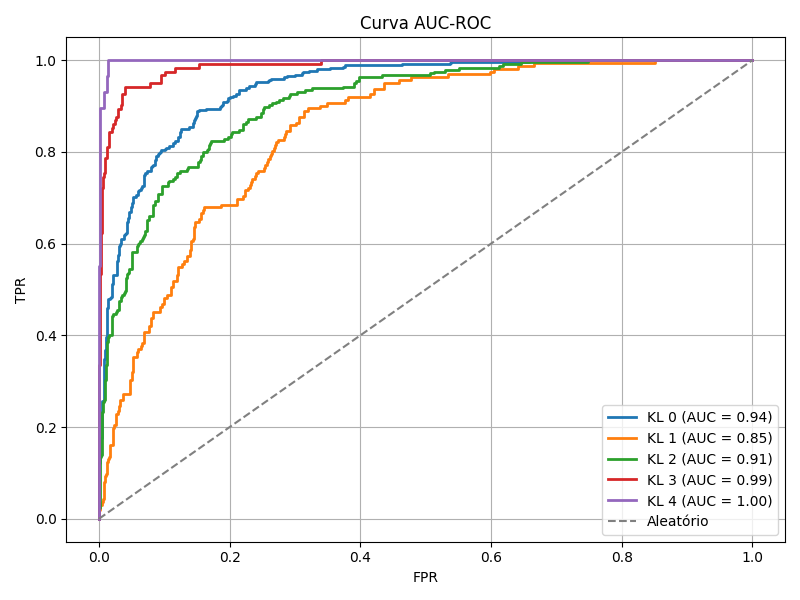
\includegraphics[width=0.38\textwidth]{figs/auc_roc/densenet169_auc_roc_cross_entropy.png} & 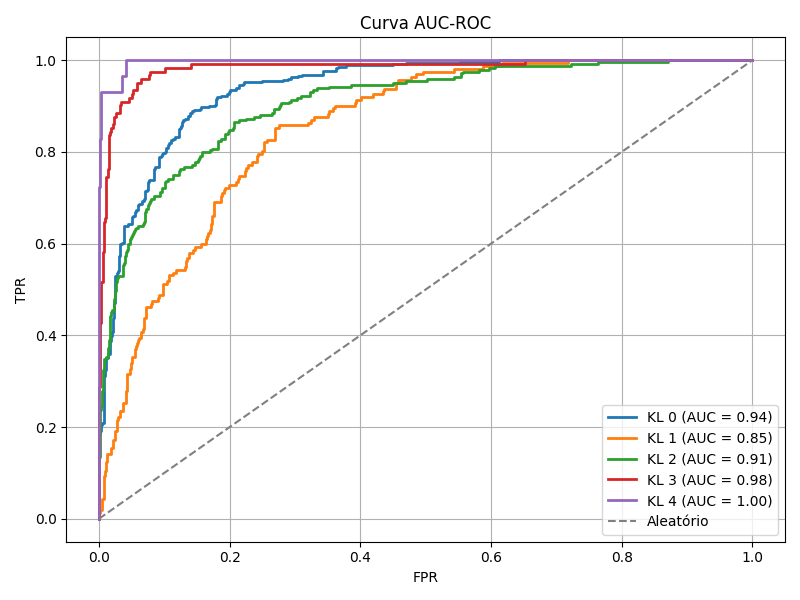
\includegraphics[width=0.38\textwidth]{figs/auc_roc/densenet169_auc_roc_corn.png} \\ \hline
        DenseNet-121 & 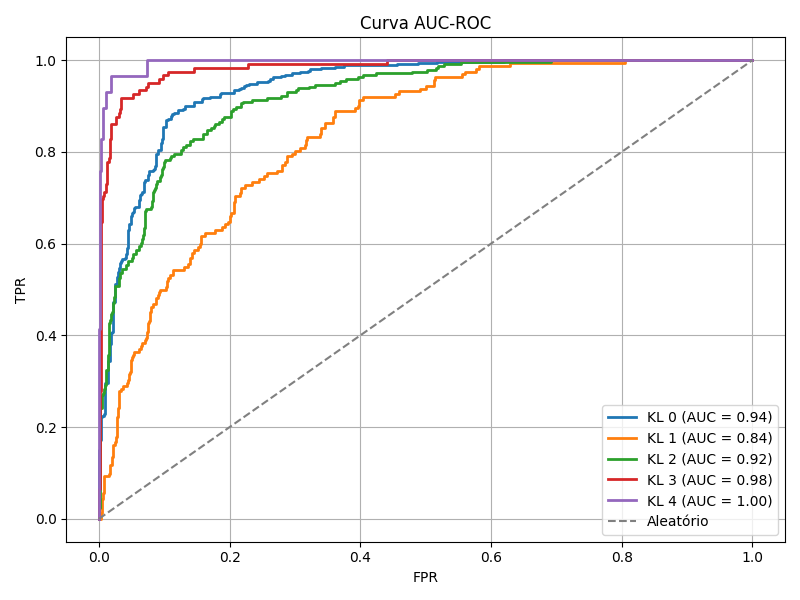
\includegraphics[width=0.38\textwidth]{figs/auc_roc/densenet121_auc_roc_cross_entropy.png} & 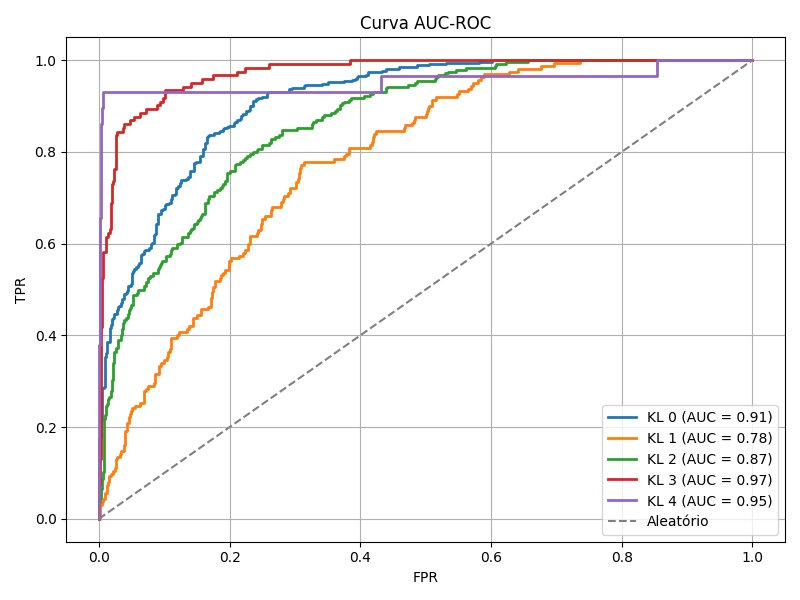
\includegraphics[width=0.38\textwidth]{figs/auc_roc/densenet121_auc_roc_corn.png} \\ \hline
        DaViT-B & 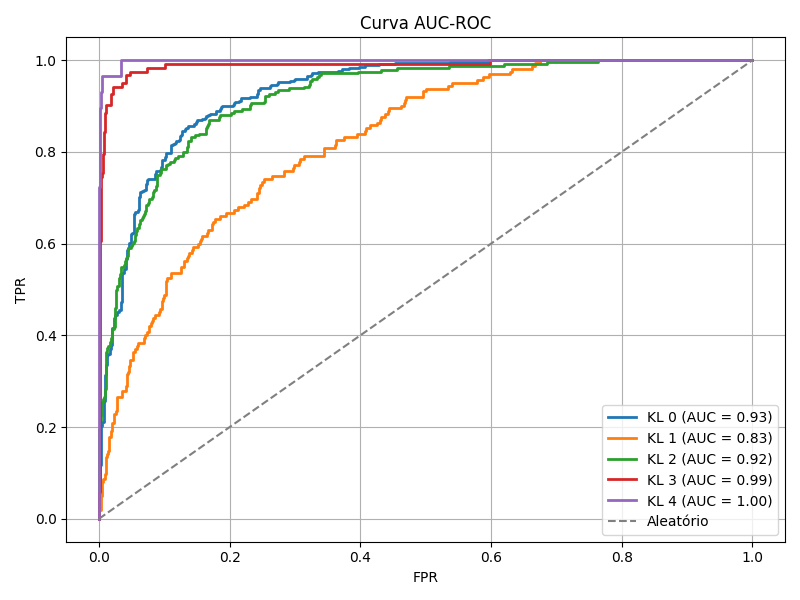
\includegraphics[width=0.38\textwidth]{figs/auc_roc/davit_base-msft_in1k_auc_roc_cross_entropy.png} & 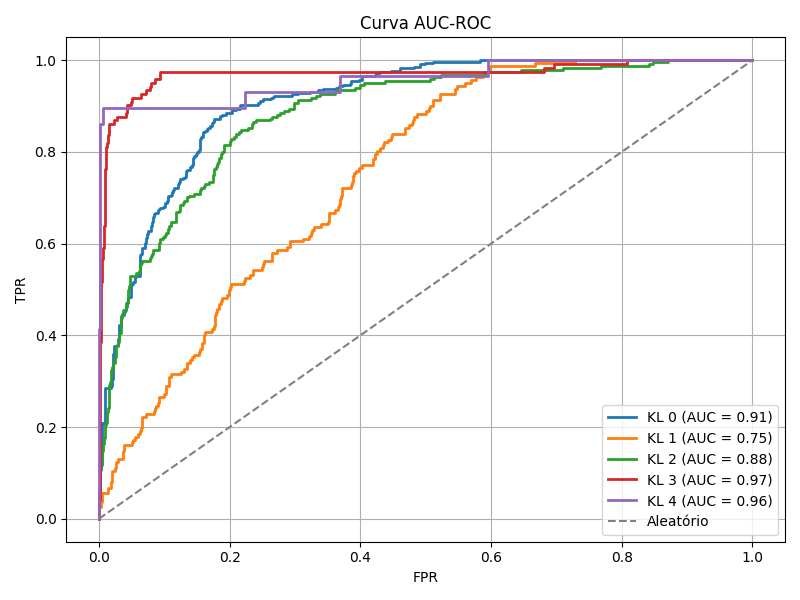
\includegraphics[width=0.38\textwidth]{figs/auc_roc/davit_base-msft_in1k_auc_roc_corn.png} \\ \hline
        GCViT-B & 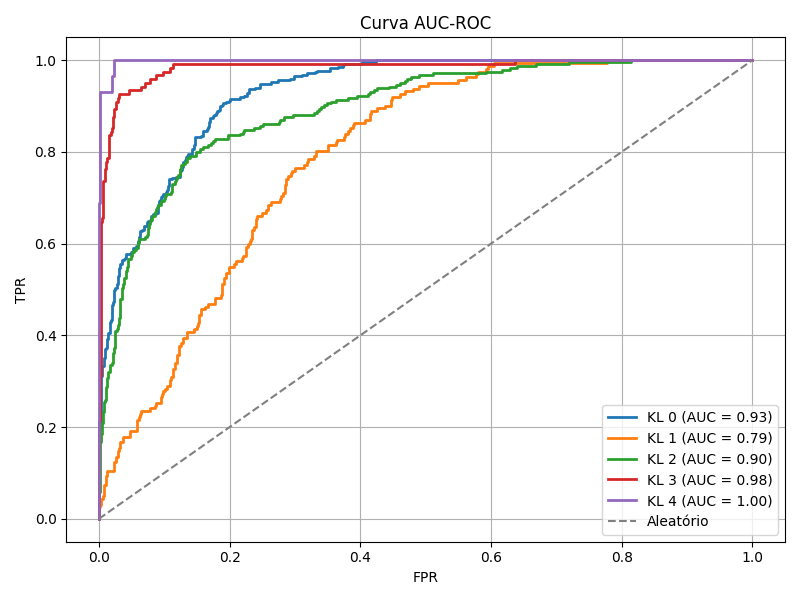
\includegraphics[width=0.38\textwidth]{figs/auc_roc/gcvit_base-in1k_auc_roc_cross_entropy.png} & 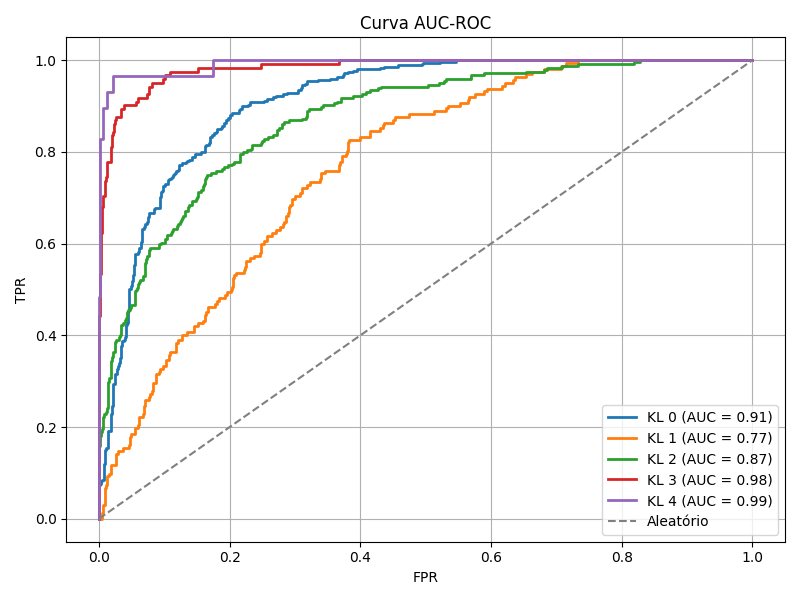
\includegraphics[width=0.38\textwidth]{figs/auc_roc/gcvit_base-in1k_auc_roc_corn.png} \\ \hline
        Inception-v3 & 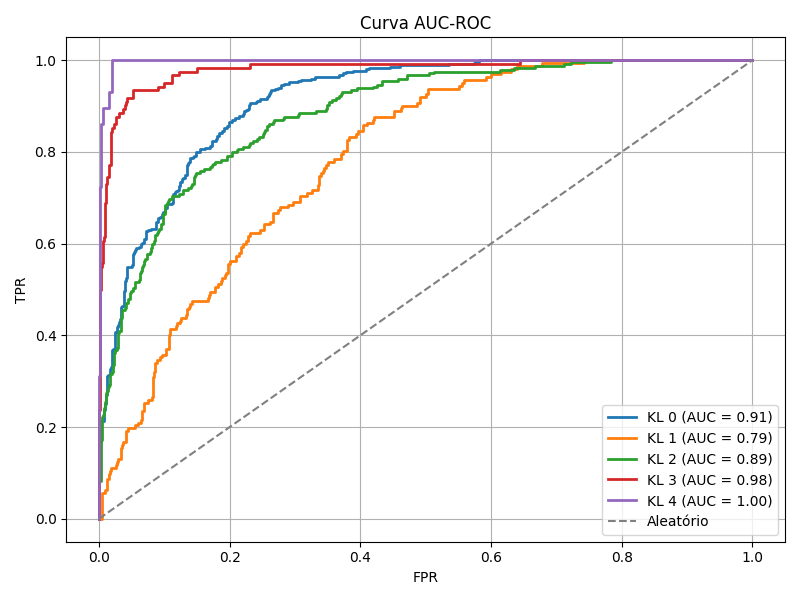
\includegraphics[width=0.38\textwidth]{figs/auc_roc/inception_v3_auc_roc_cross_entropy.png} & 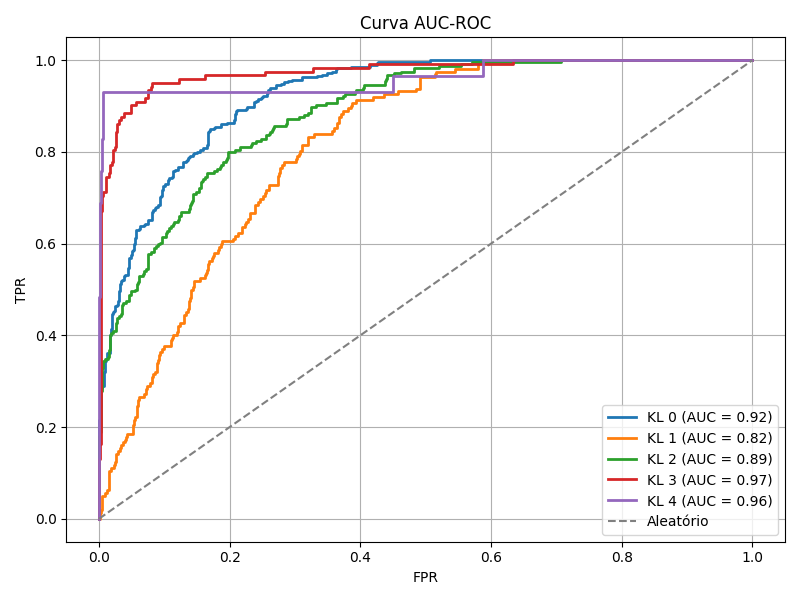
\includegraphics[width=0.38\textwidth]{figs/auc_roc/inception_v3_auc_roc_corn.png} \\ \hline
    \end{tabular}
    \caption{Curvas AUC-ROC para os cinco principais modelos.}
    \label{tab:curvas_auc_roc}
\end{table}

\section{Métricas de Desempenho por Classe}

A análise detalhada dos F1-scores por classe, apresentada na \autoref{tab:f1_scores_all_models}, revela padrões de desempenho que vão além da simples identificação de um modelo superior. Os resultados expõem a complexidade intrínseca da classificação da escala KL e destacam como diferentes arquiteturas respondem a cada estágio da doença.

\begin{sidewaystable}[!htbp]
    \centering
    \begin{tabular}{|l|l|c|c|c|c|c|c|}
        \hline
        \textbf{Modelo} & \textbf{Função de perda} & \textbf{Média Macro} & \textbf{KL-0} & \textbf{KL-1} & \textbf{KL-2} & \textbf{KL-3} & \textbf{KL-4} \\
        \hline
        ResNet-34 & \text{CE} & 0.7384 & 0.7932 & 0.4669 & 0.7187 & 0.8465 & 0.8667 \\
        \hline
        ResNet-34 & \text{CORN} & 0.7431 & 0.8034 & 0.5117 & 0.6837 & 0.8354 & 0.8814 \\
        \hline
        ResNet-50 & \text{CE} & 0.7722 & 0.7983 & 0.5257 & 0.7364 & 0.8852 & 0.9153 \\
        \hline
        ResNet-50 & \text{CORN} & 0.7564 & 0.8239 & 0.5158 & 0.7244 & 0.8326 & 0.8852 \\
        \hline
        ResNet-101 & \text{CE} & 0.7726 & 0.7983 & 0.5683 & 0.7277 & 0.8534 & 0.9153 \\
        \hline
        ResNet-101 & \text{CORN} & 0.7359 & 0.8142 & 0.4932 & 0.6920 & 0.8412 & 0.8387 \\
        \hline
        VGG-16 & \text{CE} & 0.7276 & 0.8063 & 0.4201 & 0.6912 & 0.8537 & 0.8667 \\
        \hline
        VGG-16 & \text{CORN} & 0.7384 & 0.7935 & 0.4358 & 0.7042 & 0.8583 & 0.9000 \\
        \hline
        VGG-19 & \text{CE} & 0.7066 & 0.7898 & 0.3750 & 0.7146 & 0.8468 & 0.8070 \\
        \hline
        VGG-19 & \text{CORN} & 0.7268 & 0.7935 & 0.4216 & 0.6949 & 0.8667 & 0.8571 \\
        \hline
        DenseNet-121 & \text{CE} & 0.7777 & \textbf{0.8454} & 0.5378 & 0.7537 & 0.8807 & 0.8710 \\
        \hline
        DenseNet-121 & \text{CORN} & 0.7563 & 0.8192 & 0.4890 & 0.7292 & 0.8439 & 0.9000 \\
        \hline
        DenseNet-169 & \text{CE} & \textbf{0.8061} & 0.8384 & \textbf{0.5970} & 0.7780 & 0.9016 & 0.9153 \\
        \hline
        DenseNet-169 & \text{CORN} & 0.7583 & 0.8066 & 0.5433 & 0.7097 & 0.8608 & 0.8710 \\
        \hline
        Inception-v3 & \text{CE} & 0.7487 & 0.7959 & 0.4734 & 0.7166 & 0.8455 & 0.9123 \\
        \hline
        Inception-v3 & \text{CORN} & 0.7811 & 0.8067 & 0.5464 & 0.7589 & 0.8780 & 0.9153 \\
        \hline
        DeiT-Distilled-B & \text{CE} & 0.7206 & 0.7670 & 0.3938 & 0.6790 & 0.8631 & 0.9000 \\
        \hline
        DeiT-Distilled-B & \text{CORN} & 0.7378 & 0.7527 & 0.4230 & 0.7157 & 0.8852 & 0.9123 \\
        \hline
        DaViT-B & \text{CE} & 0.7968 & 0.8111 & 0.5401 & \textbf{0.7807} & \textbf{0.9212} & \textbf{0.9310} \\
        \hline
        DaViT-B & \text{CORN} & 0.7622 & 0.7912 & 0.4756 & 0.7510 & 0.8807 & 0.9123 \\
        \hline
        MaxViT-T & \text{CE} & 0.7649 & 0.8329 & 0.4986 & 0.7143 & 0.8787 & 0.9000 \\
        \hline
        MaxViT-T & \text{CORN} & 0.7728 & 0.8333 & 0.4945 & 0.7100 & 0.8952 & \textbf{0.9310} \\
        \hline
        GCViT-B & \text{CE} & 0.7720 & 0.8409 & 0.5128 & 0.7136 & 0.8926 & 0.9000 \\
        \hline
        GCViT-B & \text{CORN} & 0.7459 & 0.8093 & 0.4501 & 0.7463 & 0.8760 & 0.8475 \\
        \hline
        Swin-B & \text{CE} & 0.7237 & 0.7944 & 0.4037 & 0.6795 & 0.8595 & 0.8814 \\
        \hline
        Swin-B & \text{CORN} & 0.7261 & 0.7994 & 0.4261 & 0.6681 & 0.8405 & 0.8966 \\
        \hline
    \end{tabular}
    \caption{Métrica F1-score para cada uma das cinco classes e modelo, considerando as funções de perda Entropia Cruzada e CORN.}
    \label{tab:f1_scores_all_models}
\end{sidewaystable}

A tabela revela a observação central onde o desempenho dos modelos é consistentemente baixo na classe KL-1 (duvidoso). Nenhum modelo, independentemente da arquitetura ou da função de perda, consegui superar um F1-score de 0,6000 para esta classe, com o melhor sendo o DenseNet-169 (0,5970) e o pior sendo o VGG-19 (0,3750). Esse resultado sugere que a classe KL-1 é inerentemente ambígua e inconsistente, assim como diz \cite{Spector1993}. Ela representa um estágio da OA onde os achados radiológicos, como um possível estreitamento do espaço articular ou a formação de osteófitos, são muito sutis. Como consequência, essa classe sofre com a sobreposição de características entre as classes adjacentes, tornando a classificação pelos modelos mais desafiadora. Esse padrão é visualmente confirmado nas matrizes de confusão apresentadas na \autoref{tab:matrizes_confusao}, onde observa-se um número elevado de classificações incorretas entre as classes KL-1 e as classes adjacentes KL-0 e KL-2.

\begin{table}[!htbp]
    \centering
    \begin{tabular}{|c|c|c|}
        \hline
        \textbf{Modelo} & \textbf{CE} & \textbf{CORN} \\ \hline
        DenseNet-169 & 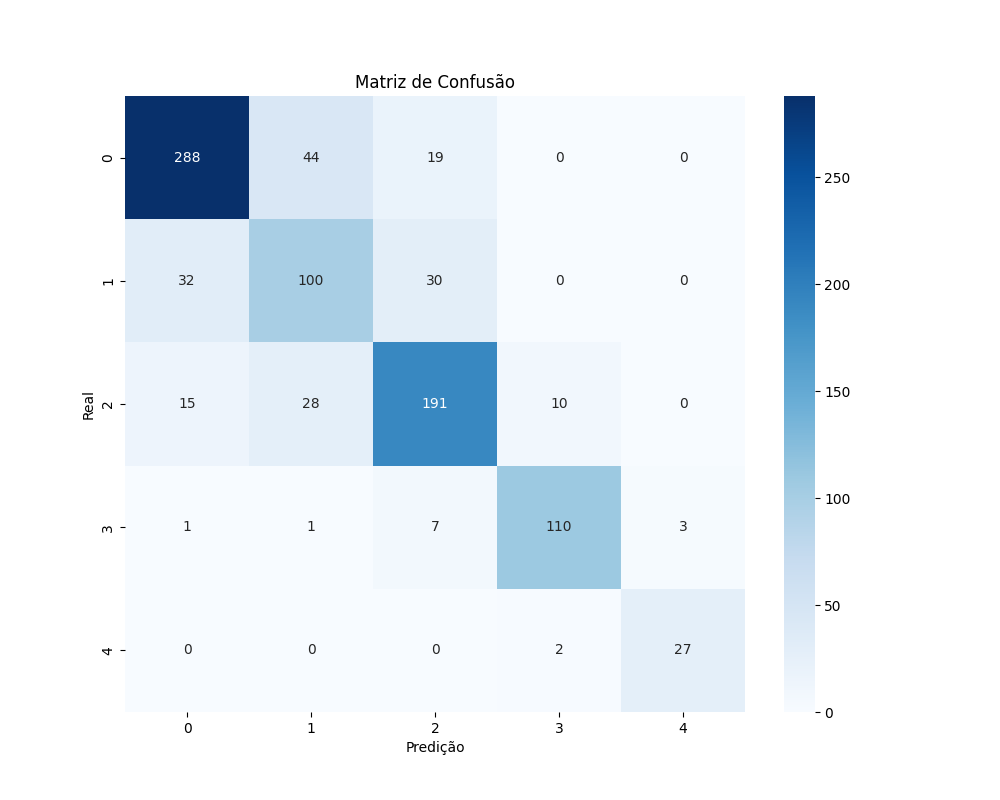
\includegraphics[width=0.37\textwidth]{figs/confusion_matrices/densenet169_cm_cross_entropy.png} & 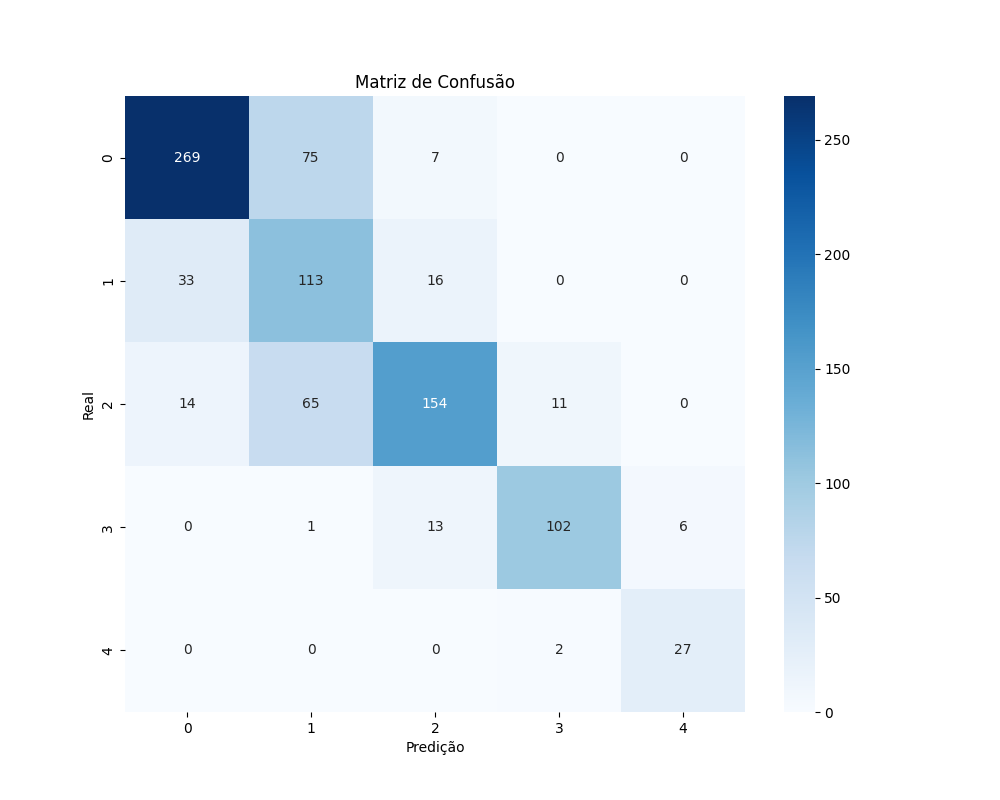
\includegraphics[width=0.37\textwidth]{figs/confusion_matrices/densenet169_cm_corn.png} \\ \hline
        DenseNet-121 & 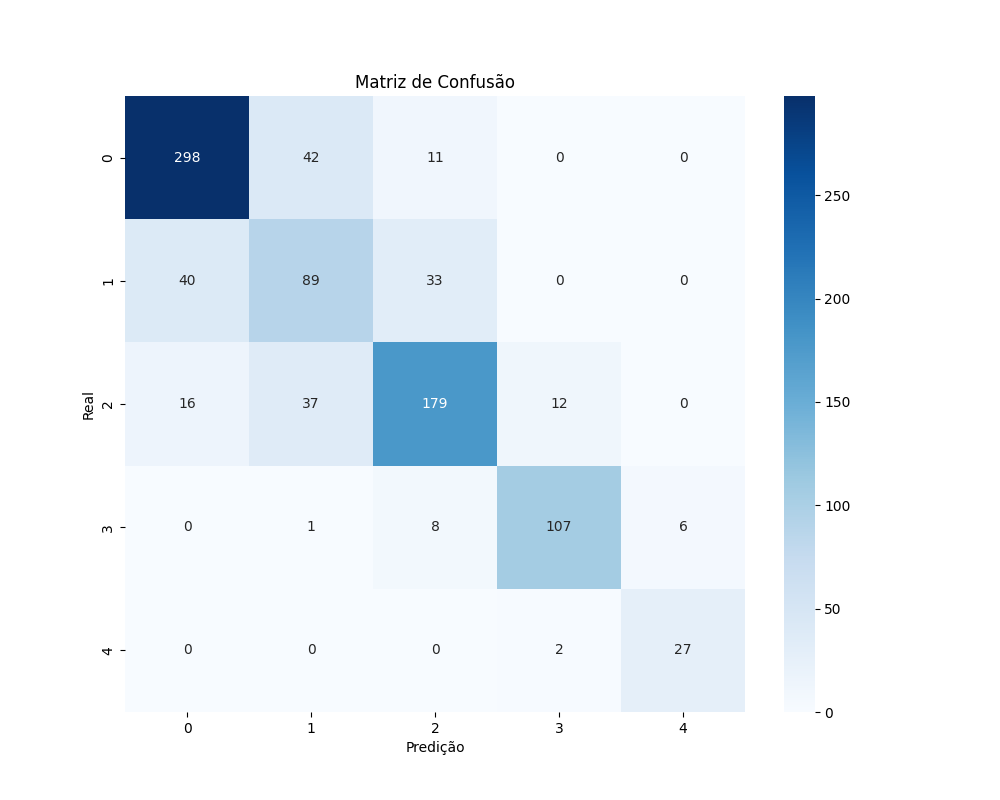
\includegraphics[width=0.37\textwidth]{figs/confusion_matrices/densenet121_cm_cross_entropy.png} & 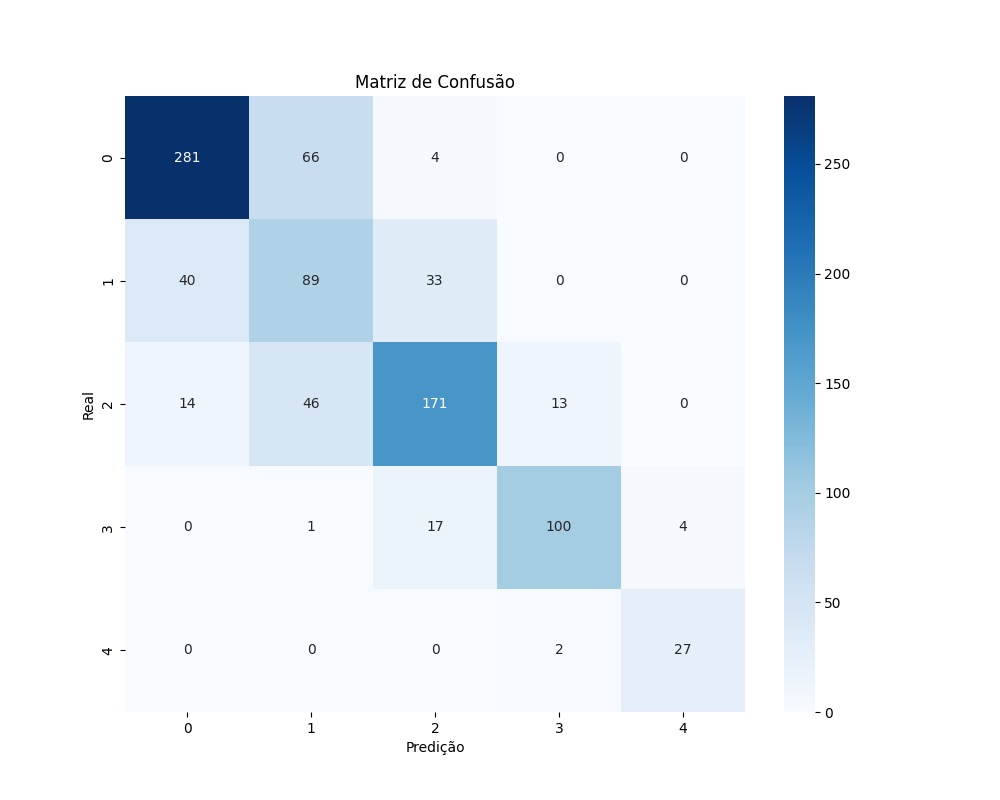
\includegraphics[width=0.37\textwidth]{figs/confusion_matrices/densenet121_cm_corn.png} \\ \hline
        DaViT-B & 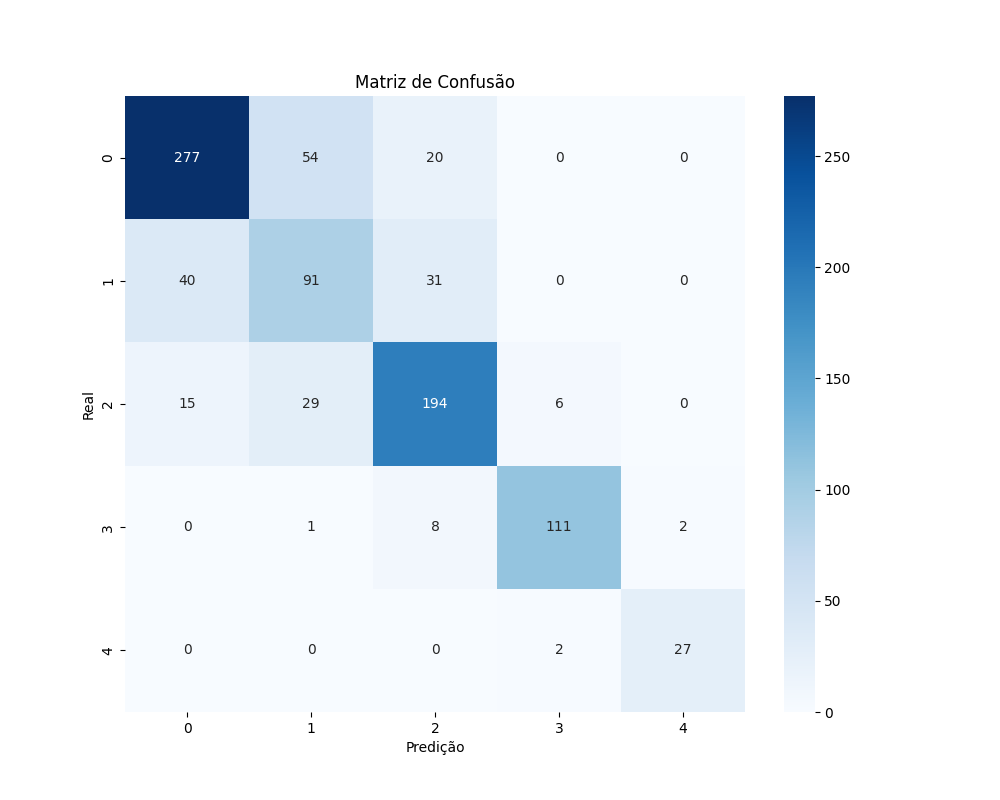
\includegraphics[width=0.37\textwidth]{figs/confusion_matrices/davit_base-msft_in1k_cm_cross_entropy.png} & 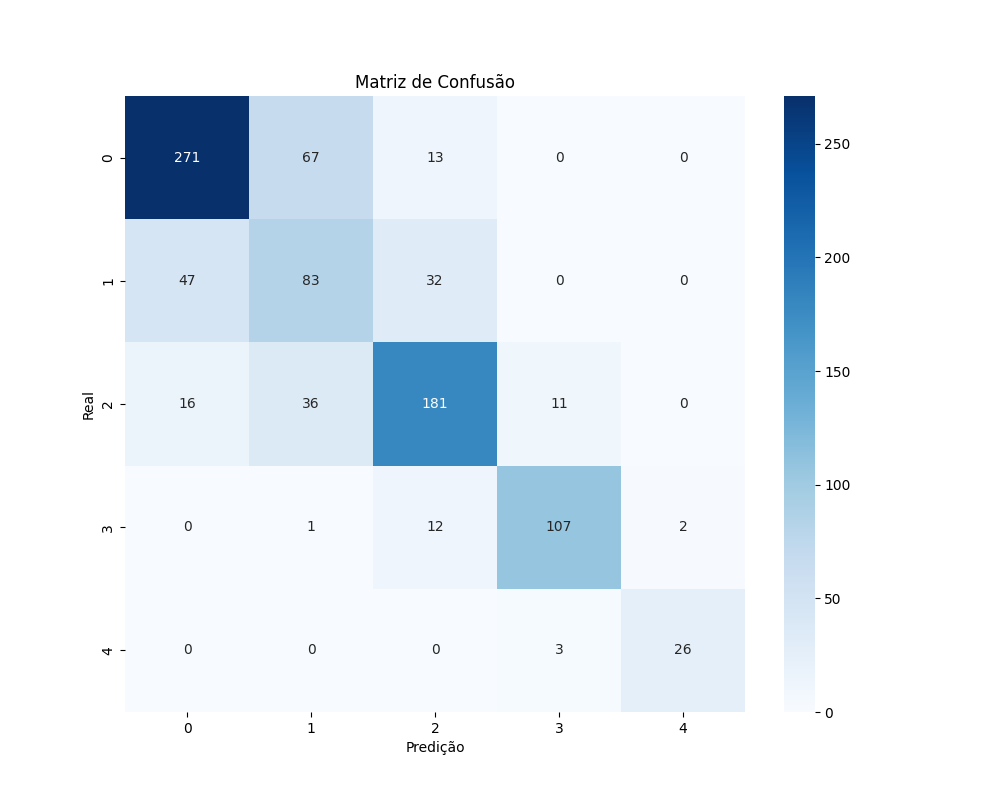
\includegraphics[width=0.37\textwidth]{figs/confusion_matrices/davit_base-msft_in1k_cm_corn.png} \\ \hline
        GCViT-B & 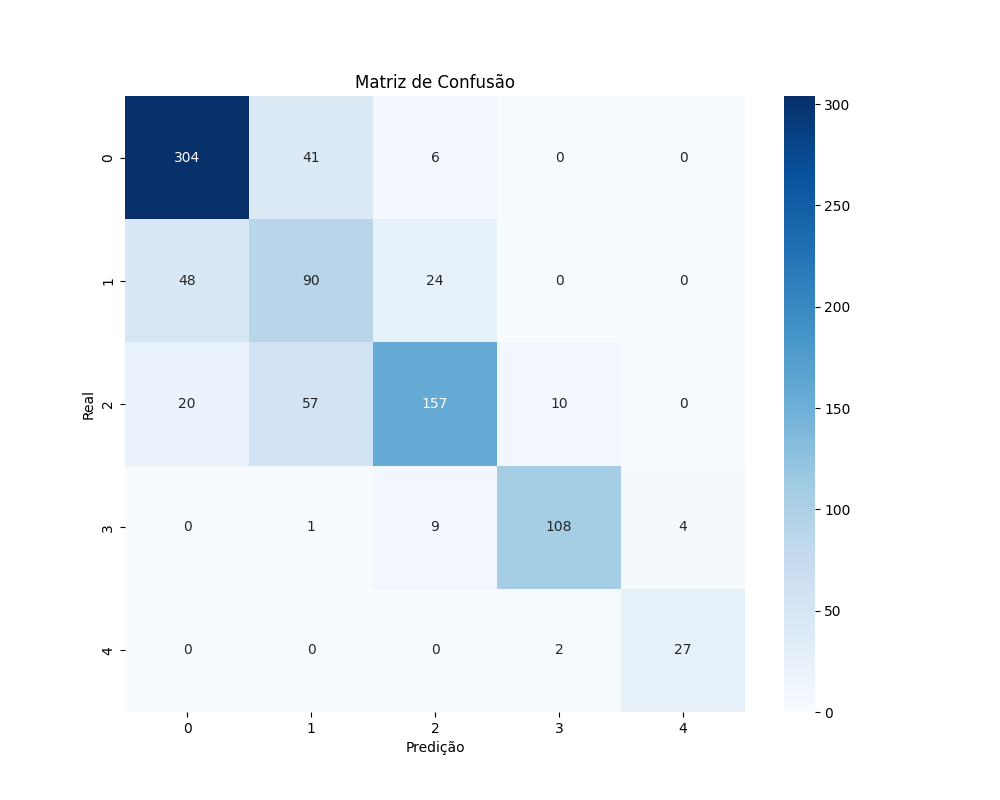
\includegraphics[width=0.37\textwidth]{figs/confusion_matrices/gcvit_base-in1k_cm_cross_entropy.png} & 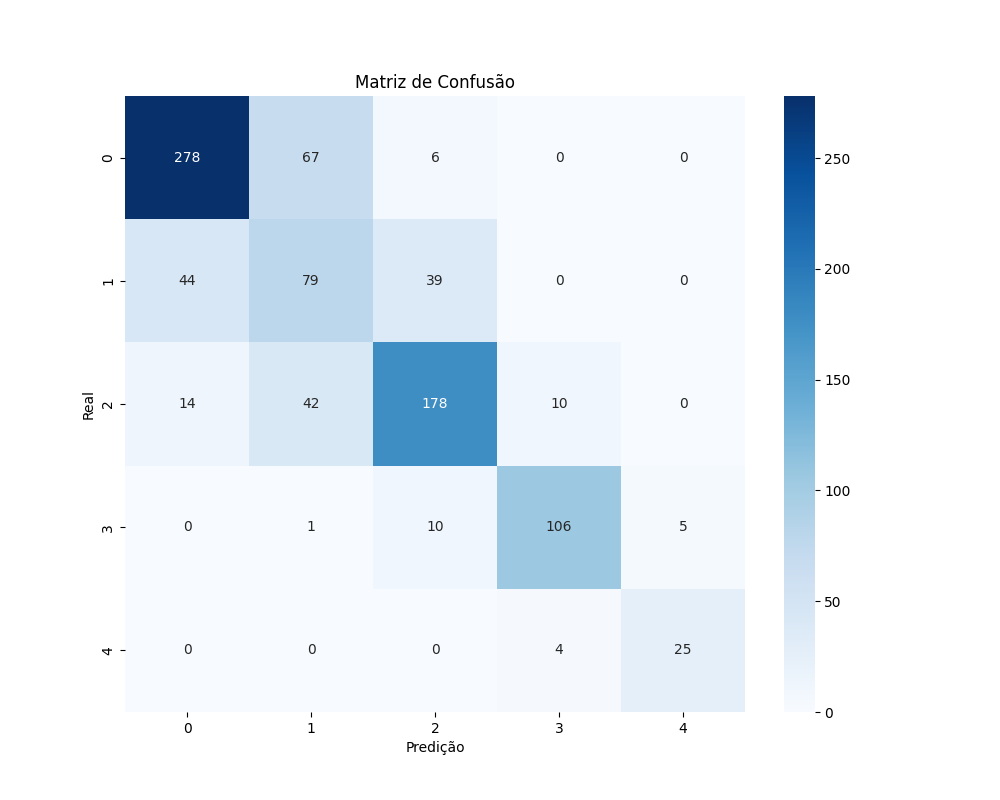
\includegraphics[width=0.37\textwidth]{figs/confusion_matrices/gcvit_base-in1k_cm_corn.png} \\ \hline
        Inception-v3 & 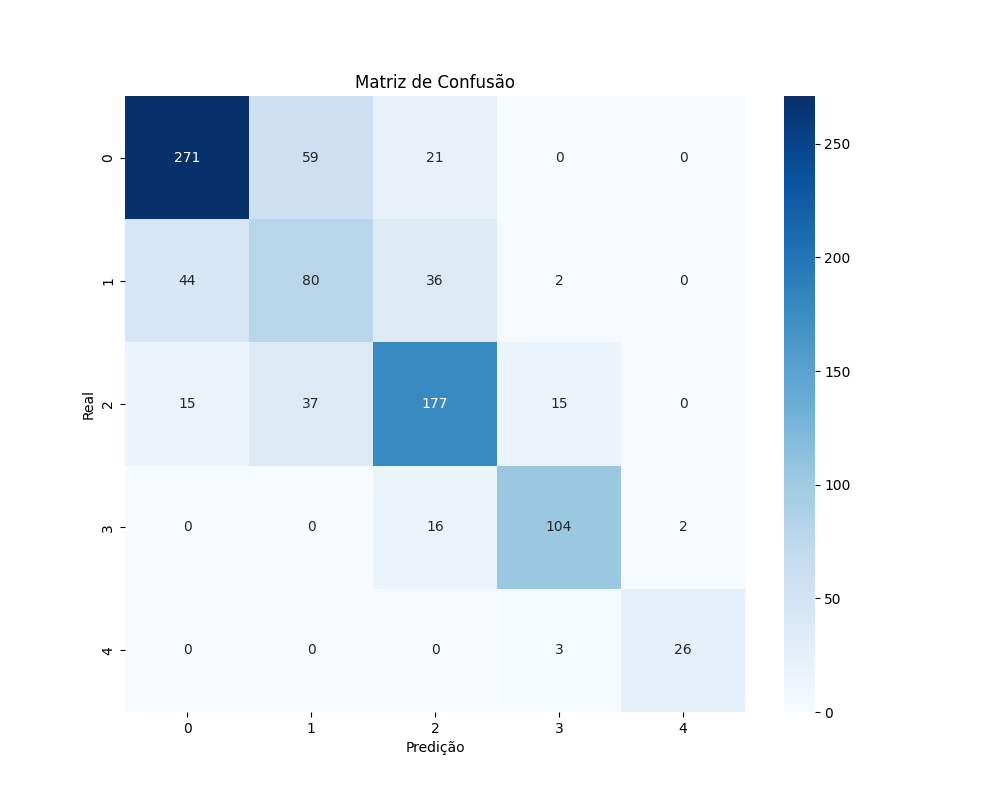
\includegraphics[width=0.37\textwidth]{figs/confusion_matrices/inception_v3_cm_cross_entropy.png} & 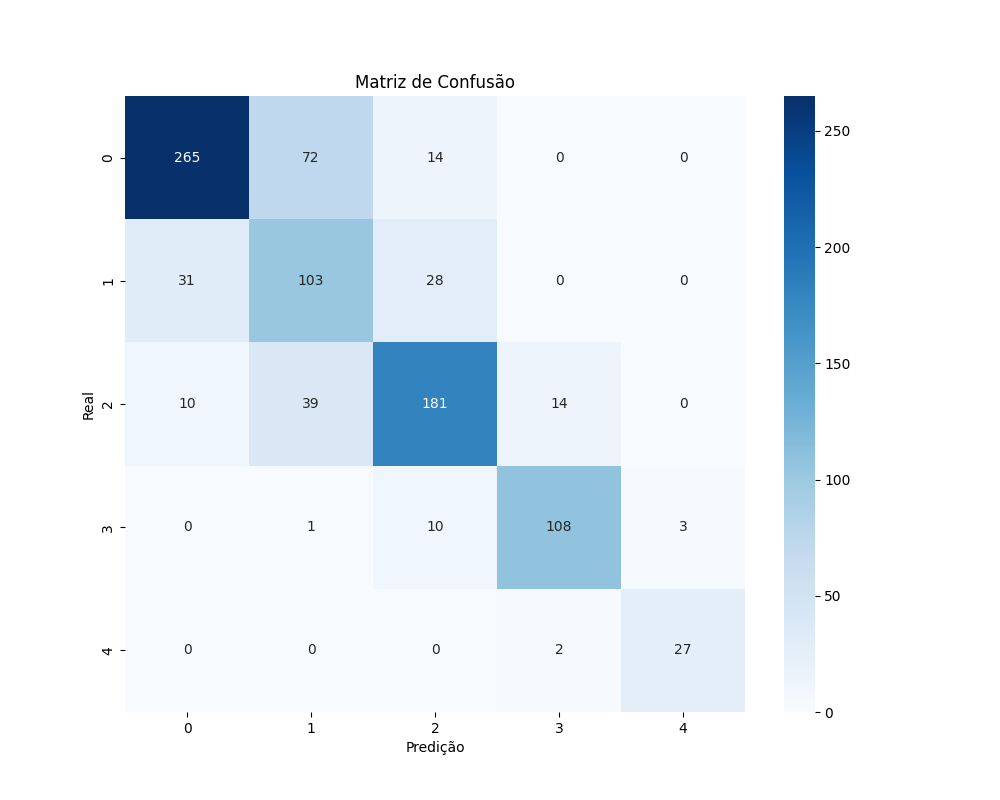
\includegraphics[width=0.37\textwidth]{figs/confusion_matrices/inception_v3_cm_corn.png} \\ \hline
    \end{tabular}
    \caption{Matriz de confusão para os cinco principais modelos.}
    \label{tab:matrizes_confusao}
\end{table}

Em forte contraste com a classe KL-1, as classes nos extremos da escala, KL-0 (saudável) e KL-4 (severo), apresentam F1-scores consistentemente altos na maioria dos modelos. Para a classe KL-0, modelos como DenseNet-121 (0,8454) e GCViT-B (0,8409) demostraram uma boa capacidade de identificar corretamente um joelho saudável. Já para a classe KL-4, os resultados são ainda mais expressivos, com modelos como DaViT-B e MaxViT-T alcançando F1-scores muito elevados, ambos com 0,9310.

As classes KL-2 (mínimo) e KL-3 (moderado) representam estágios onde a doença já está presente e o desempenho dos modelos foi mais equilibrado. Modelos como DaViT-B (0,9212 para KL-3) e DenseNet-169 (0,9016 para KL-3) mostraram uma capacidade notável de distinguir os estágios intermediários da doença.

Essa análise por classe não apenas valida a decisão de realizar experimentos excluindo a classe KL-1, mas também confirma que o desempenho dos modelos está fortemente alinhado à realidade clínica da OA de joelho, onde existe uma alta certeza nos casos extremos e dificuldade na zona de transição (por exemplo, a classe KL-1).

\section{Comparações com Trabalhos Relacionados}

O desempenho do melhor modelo deste estudo (DenseNet-169) foi comparado com trabalhos recentes da literatura que abordam a mesma tarefa de classificação da severidade da OA de joelho. A \autoref{tab:study_comparisons} resume essa comparação. É importante ressaltar que uma comparação direta entre estudos pode ser desafiadora devido a variações em protocolos experimentais, como o conjunto de dados utilizado, as técnicas de pré-processamento e o hardware utilizado. Apesar dessas variações, a análise indica que os resultados deste estudo são altamente competitivos e, em métricas cruciais, superiores à maioria dos trabalhos recentes, especialmente quando se considera uma avaliação holística do desempenho.

\begin{table}[!htbp]
    \centering
    \begin{tabular}{|c|c|c|c|c|c|}
        \hline
        \textbf{Referência} & \textbf{Número de Classes} & \textbf{Acurácia} & \textbf{QWK} & \textbf{F1-score} & \textbf{AUC} \\
        \hline
        \cite{Tariq2023} & 5 & \makecell{98,00\%} & \makecell{0,990} & \makecell{0,980} & \makecell{0,970} \\
        \hline
        \cite{Mohammed2023} & 5 & \makecell{69,00\%} & \makecell{-} & \makecell{0,670} & \makecell{-} \\
        \hline
        \cite{domingues2023} & 2 & \makecell{90,70\%} & \makecell{-} & \makecell{0,553} & \makecell{0,866} \\
        \hline
        \cite{Cueva2022} & 5 & \makecell{61,71\%} & \makecell{-} & \makecell{-} & \makecell{-} \\
        \hline
        \cite{yeoh2023} & 2 & \makecell{87,50\%} & \makecell{-} & \makecell{0,871} & \makecell{0,945} \\
        \hline
        \cite{sekhri2023} & 5 & \makecell{70,17\%} & \makecell{-} & \makecell{0,671} & \makecell{-} \\
        \hline
        \cite{Wang_2024} & 2 & \makecell{89,90\%} & \makecell{-} & \makecell{0,877} & \makecell{-} \\
        \hline
        \cite{apon2024} & 5 & \makecell{66,14\%} & \makecell{-} & \makecell{0,618} & \makecell{0,860} \\
        \hline
        Este estudo & 5 & \makecell{78,85\%} & \makecell{0,888} & \makecell{0,806} & \makecell{0,938} \\
        \hline
    \end{tabular}
    \caption{Comparação entre os resultados de diferentes estudos que abordam o mesmo problema.}
    \label{tab:study_comparisons}
\end{table}

Ao analisar os trabalhos que consideram as cinco classes KL, observa-se que o presente estudo, com 78,85\% de acurácia, supera significativamente os resultados de \cite{Mohammed2023} (69,00\%), \cite{Cueva2022} (61,71\%), \cite{sekhri2023} (70,17\%) e \cite{apon2024} (66,14\%). A superioridade é particularmente evidente no F1-score (0,806), que indica um melhor equilíbrio entre precisão e revocação entre todas as cinco classes em comparação com os valores reportados por \cite{Mohammed2023} (0,670) e \cite{apon2024} (0,618). O trabalho de \cite{Tariq2023} apresenta resultados excepcionalmente elevados (98,00\% de acurácia), que foram obtidos a partir de um modelo \textit{ensemble}, além desse resultado ser atribuído a um subconjunto de dados menos desafiador ou protocolos de validação que podem não garantir uma separação estrita entre treino e teste.

Um diferencial significativo deste estudo é a avaliação através de métricas mais alinhadas à natureza do problema. O QWK de 0,888 demonstra não apenas que o modelo é acurado, mas que seus erros são, em sua maioria, clinicamente menos graves (próximos da classe real), uma análise de robustez que está ausente na maioria dos trabalhos comparados. Da mesma forma, o valor de AUC de 0,938 indica uma excelente capacidade de separação entre as classes, superando os valores reportados por \cite{domingues2023} (0,866) e \cite{apon2024} (0,860).

Portanto, embora alguns estudos possam apresentar valores de acurácia isoladamente mais altos, os resultados aqui obtidos demonstram um desempenho mais robusto, equilibrado e rigorosamente avaliado. O modelo deste estudo não apenas supera a maioria dos trabalhos em métricas padrão, mas também se destaca em métricas ordinais e de separabilidade de classes, estabelecendo um \textit{benchmark} sólido e confiável para a classificação da OA de joelho em cinco classes.

\section{Eficiência Computacional}

A análise dos tempos de treinamento e inferência, apresentada na \autoref{tab:computational_performance}, revela distinções cruciais entre os modelos e funções de perda, oferecendo um respaldo da aplicação prática e que complementa as métricas de desempenho preditivo.

O tempo de inferência por imagem é uma métrica crítica para a aplicação clínica, e as RNCs demonstram uma vantagem sobre os ViTs. Modelos como ResNet-34 (1,55 ms/imagem), ResNet-50 (2,87 ms/imagem) e DenseNet/121 (3,11 ms/imagem) são os mais rápidos, estabelecendo uma linha de base de alta eficiência. Suas arquiteturas são bem otimizadas para o hardware de GPU, o que permite um processamento rápido.

Em contraste, os ViTs apresentaram tempos de inferência significativamente mais altos. O mais rápido entre eles, MaxViT-T (6,92 ms/imagem), já é mais de duas vezes mais lento do que as RNCs eficientes. Essa disparidade pode ser justificada pela natureza das operações. Embora ViTs tenham alcançado complexidade computacional linear em relação ao tamanho de imagem, como citam \cite{ding2022davitdualattentionvision} e \cite{maxvit2022}, seus blocos de atenção ainda envolvem operações de multiplicação de matrizes em larga escala que são mais custosas do que as operações de convolução. Isso também pode ser visualizado na \autoref{tab:model_list}, na coluna de FLOPs (GMac).

A literatura sobre modelos como MaxViT e DaViT foca em tornar a atenção global mais eficiente e de fato tornam, mas os resultados práticos da \autoref{tab:computational_performance} demonstram que, na GPU utilizada, a sobrecarga computacional da auto-atenção ainda é um obstáculo significativo para a inferência quando comparada às RNCs.

\begin{sidewaystable}[!htbp]
    \centering
    \begin{tabular}{|l|l|c|c|c|}
        \hline
        \textbf{Modelo} & \textbf{Função de perda} & \textbf{Treinamento (\textit{min})} & \textbf{Inferência média/batch (\textit{ms})} & \textbf{Inferência média/imagem (\textit{ms})} \\
        \hline
        ResNet-34 & CE & 33,46 & \textbf{43,53} & \textbf{1,55} \\
        \hline
        ResNet-34 & CORN & 89,29 & 43,71 & 1,56 \\
        \hline
        ResNet-50 & CE & 14,55 & 80,45 & 2,87 \\
        \hline
        ResNet-50 & CORN & 9,87 & 80,83 & 2,89 \\
        \hline
        ResNet-101 & CE & 22,02 & 137,90 & 4,93 \\
        \hline
        ResNet-101 & CORN & 16,94 & 139,76 & 4,99 \\
        \hline
        VGG-16 & CE & 37,70 & 128,08 & 4,57 \\
        \hline
        VGG-16 & CORN & 28,45 & 126,44 & 4,52 \\
        \hline
        VGG-19 & CE & 39,32 & 153,06 & 5,47 \\
        \hline
        VGG-19 & CORN & 34,68 & 154,96 & 5,53 \\
        \hline
        DenseNet-121 & CE & 12,74 & 87,02 & 3,11 \\
        \hline
        DenseNet-121 & CORN & \textbf{9,22} & 87,26 & 3,12 \\
        \hline
        DenseNet-169 & CE & 15,06 & 108,95 & 3,89 \\
        \hline
        DenseNet-169 & CORN & 16,72 & 108,48 & 3,87 \\
        \hline
        Inception-v3 & CE & 12,52 & 108,58 & 3,88 \\
        \hline
        Inception-v3 & CORN & 14,39 & 108,86 & 3,89 \\
        \hline
        DeiT-Distilled-B & CE & 77,31 & 331,55 & 11,84 \\
        \hline
        DeiT-Distilled-B & CORN & 40,20 & 330,48 & 11,80 \\
        \hline
        DaViT-B & CE & 57,83 & 335,72 & 11,99 \\
        \hline
        DaViT-B & CORN & 27,08 & 339,09 & 12,11 \\
        \hline
        MaxViT-T & CE & 28,03 & 193,82 & 6,92 \\
        \hline
        MaxViT-T & CORN & 29,36 & 194,79 & 6,96 \\
        \hline
        GCViT-B & CE & 49,57 & 408,07 & 14,57 \\
        \hline
        GCViT-B & CORN & 34,65 & 409,04 & 14,61 \\
        \hline
        Swin-B & CE & 46,61 & 344,37 & 12,30 \\
        \hline
        Swin-B & CORN & 36,02 & 348,65 & 12,45 \\
        \hline
    \end{tabular}
    \caption{Tempos de treinamento e inferência de cada modelo.}
    \label{tab:computational_performance}
\end{sidewaystable}

\section{Análise Quantitativa}

A predição conformal foi aplicada para quantificar a incerteza dos modelos, gerando conjuntos de predição com um nível de confiança estatisticamente garantido de 95\%. A análise dos resultados, apresentados na \autoref{tab:conformal_coverage}, sugere uma compensação entre a robustez da garantia de cobertura e a utilidade prática dos conjuntos de predição, com diferenças expressivas entre a abordagem padrão e a ordinal.

\begin{table}[!htbp]
    \centering
    \begin{tabular}{|l|l|c|}
        \hline
        \textbf{Modelo} & \textbf{Função de perda} & \textbf{Cobertura} \\
        \hline
        ResNet-34 & CE &    0,9989 \\
        \hline
        ResNet-34 & CORN &    0,8822 \\
        \hline
        ResNet-50 & CE &    \textbf{1,0000} \\
        \hline
        ResNet-50 & CORN &    0,9361 \\
        \hline
        ResNet-101 & CE &    0,9956 \\
        \hline
        ResNet-101 & CORN &    0,8844 \\
        \hline
        VGG-16 & CE &    \textbf{1,0000} \\
        \hline
        VGG-16 & CORN &    0,9273 \\
        \hline
        VGG-19 & CE &    0,9989 \\
        \hline
        VGG-19 & CORN &    0,9262 \\
        \hline
        DenseNet-121 & CE &    \textbf{1,0000} \\
        \hline
        DenseNet-121 & CORN &    0,8667 \\
        \hline
        DenseNet-169 & CE &    0,9989 \\
        \hline
        DenseNet-169 & CORN &    0,9163 \\
        \hline
        Inception-v3 & CE &    0,9989 \\
        \hline
        Inception-v3 & CORN &    0,9416 \\
        \hline
        DeiT-Distilled-B & CE &    \textbf{1,0000} \\
        \hline
        DeiT-Distilled-B & CORN &    0,9163 \\
        \hline
        DaViT-B & CE &    0,9989 \\
        \hline
        DaViT-B & CORN &    0,8844 \\
        \hline
        MaxViT-T & CE &    0,9989 \\
        \hline
        MaxViT-T & CORN &    0,9031 \\
        \hline
        GCViT-B & CE &    0,9989 \\
        \hline
        GCViT-B & CORN &    0,8954 \\
        \hline
        Swin-B & CE &    \textbf{1,0000} \\
        \hline
        Swin-B & CORN &    0,8822 \\
        \hline
    \end{tabular}
    \caption{Valores de cobertura da predição conformal para cada modelo e função de perda.}
    \label{tab:conformal_coverage}
\end{table}

Como descrito na \autoref{sec:conformal-prediction}, a cobertura mede a porcentagem de vezes que a classe verdadeira esteve contida no conjunto de predição conformal a partir das imagens de teste. Modelos treinados com entropia cruzada demonstraram uma cobertura muito alta, consistentemente alcançando valores de 100\%, como é o caso do ResNet-50, VGG-16, DenseNet-121, DeiT-Distilled-B e Swin-B. Embora isso satisfaça a garantia teórica de cobrir pelo menos 95\% dos casos, valores altos podem indicar que o método é excessivamente conservador, ou seja, que o limiar de confiança ($\hat{q}$) calculado é muito alto, levando os modelos a incluírem mais classes para garantir a cobertura.

Já a cobertura para os modelos treinados com CORN foi mais variável, geralmente situando-se mais próxima ao objetivo de 95\%, exemplo do ResNet-50 (93,61\%) e Inception-v3 (94,16\%). No entanto, alguns modelos apresentaram uma cobertura abaixo do esperado, como o DenseNet-121, com 86,67\%, indicando que a abordagem ordinal, embora mais ``justa'' em sua calibração, pode ser menos estável em garantir a cobertura em todos os casos.

Analisando agora o tamanho dos conjuntos de predição gerados, a utilidade do método da predição conformal é inversamente proporcional ao tamanho desses conjuntos, isto é, conjuntos menores indicam maior confiança e são mais informativos. Nesse sentido, a abordagem ordinal com CORN desmonstrou uma superioridade prática.

Como pode ser visto na \autoref{tab:cp_set_sizes}, os histogramas para os modelos treinados com entropia cruzada mostram uma certa tendência de incerteza, pois raramente expressam confiança suficiente para gerar uma predição única. Por exemplo, o Swin-B não gerou nenhum conjunto de tamanho um, enquanto o ResNet-50 gerou apenas cinco. A grande maioria das predições resultou em conjuntos de tamanho três ou quatro, tornando a saída pouco útil na prática. No modelo DaViT-B, 828 das 908 predições (mais de 91\%) continham três ou mais classes possíveis. Para um radiologista, um resultado como ``Grau 1, 2 ou 3'' oferece pouca orientação para diagnosticar o nível de severidade da OA.

\begin{table}[!htbp]
    \centering
    \begin{tabular}{|c|c|c|}
        \hline
        \textbf{Modelo} & \textbf{CE} & \textbf{CORN} \\ \hline
        ResNet-50 & 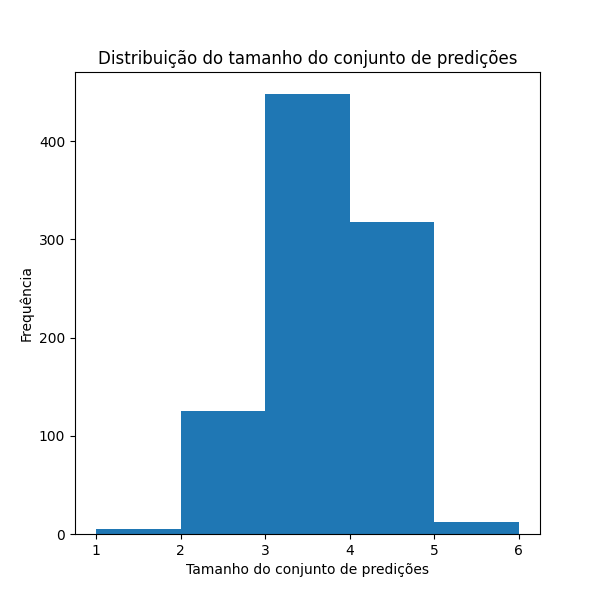
\includegraphics[width=0.25\textwidth]{figs/conformal_prediction/resnet50_cp_cross_entropy.png} & 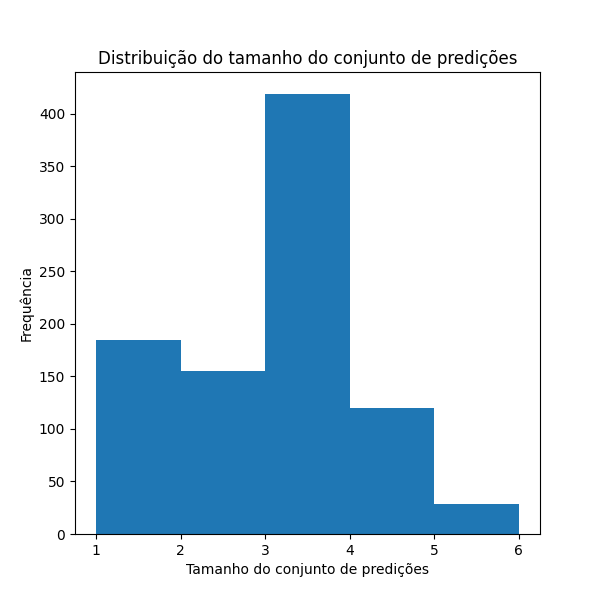
\includegraphics[width=0.25\textwidth]{figs/conformal_prediction/resnet50_cp_corn.png} \\ \hline
        Swin-B & 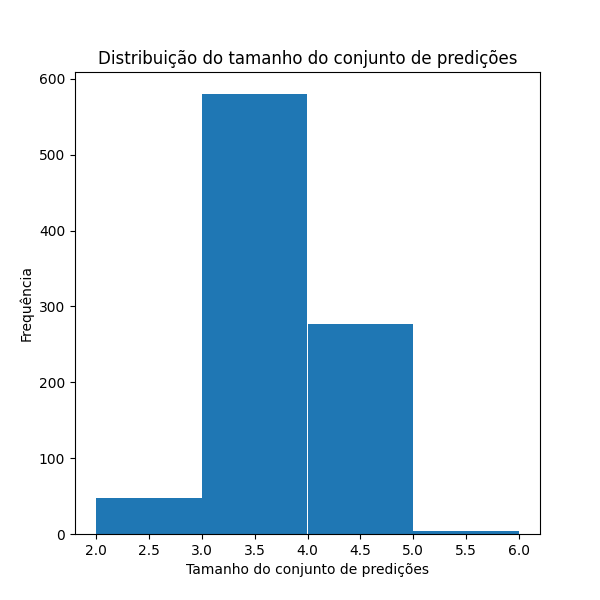
\includegraphics[width=0.25\textwidth]{figs/conformal_prediction/swin_b_cp_cross_entropy.png} & 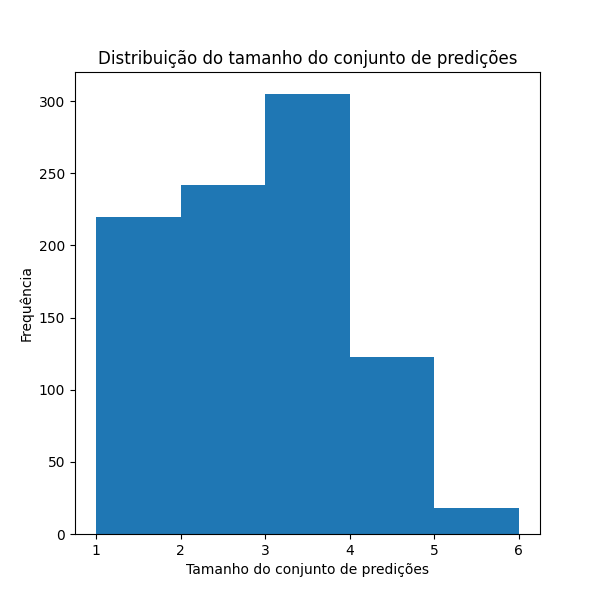
\includegraphics[width=0.25\textwidth]{figs/conformal_prediction/swin_b_cp_corn.png} \\ \hline
        Inception-v3 & 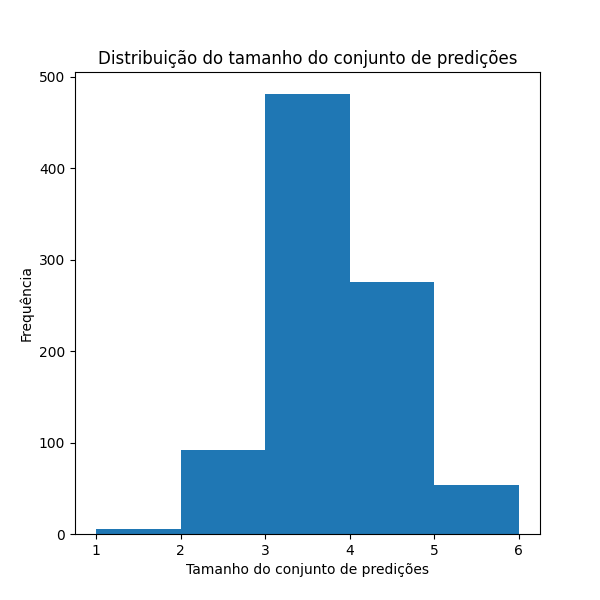
\includegraphics[width=0.25\textwidth]{figs/conformal_prediction/inception_v3_cp_cross_entropy.png} & 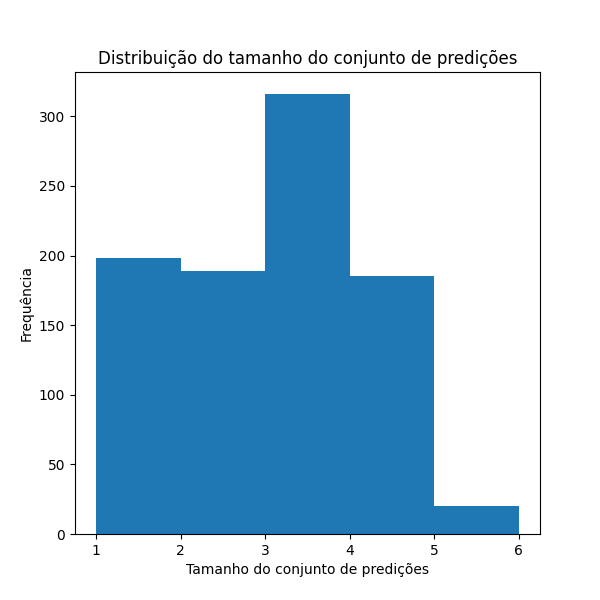
\includegraphics[width=0.25\textwidth]{figs/conformal_prediction/inception_v3_cp_corn.png} \\ \hline
        DaViT-B & 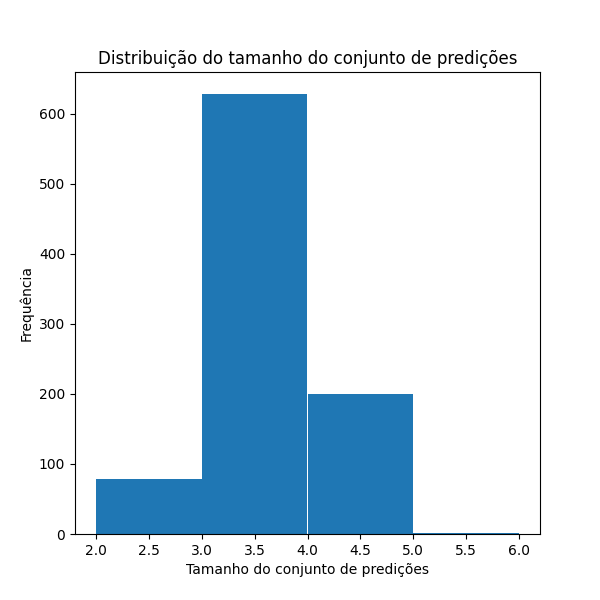
\includegraphics[width=0.25\textwidth]{figs/conformal_prediction/davit_base-msft_in1k_cp_cross_entropy.png} & 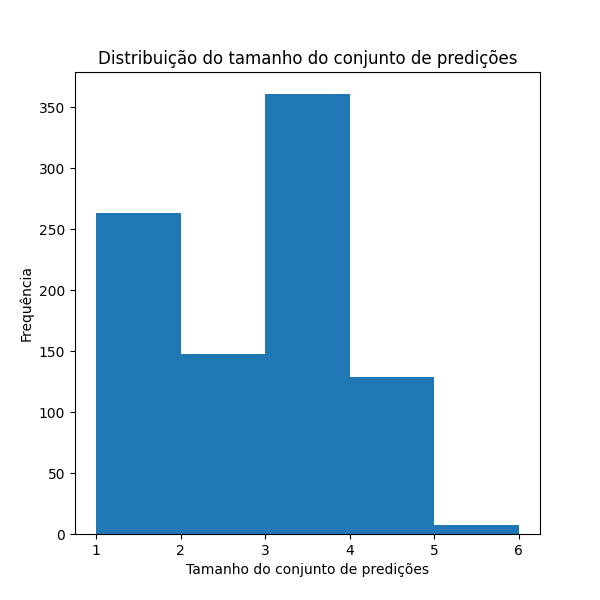
\includegraphics[width=0.25\textwidth]{figs/conformal_prediction/davit_base-msft_in1k_cp_corn.png} \\ \hline
        DenseNet-169 & 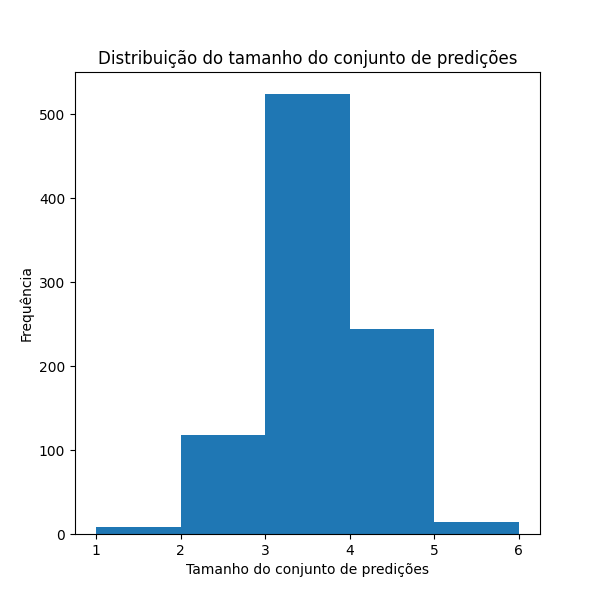
\includegraphics[width=0.25\textwidth]{figs/conformal_prediction/densenet169_cp_cross_entropy.png} & 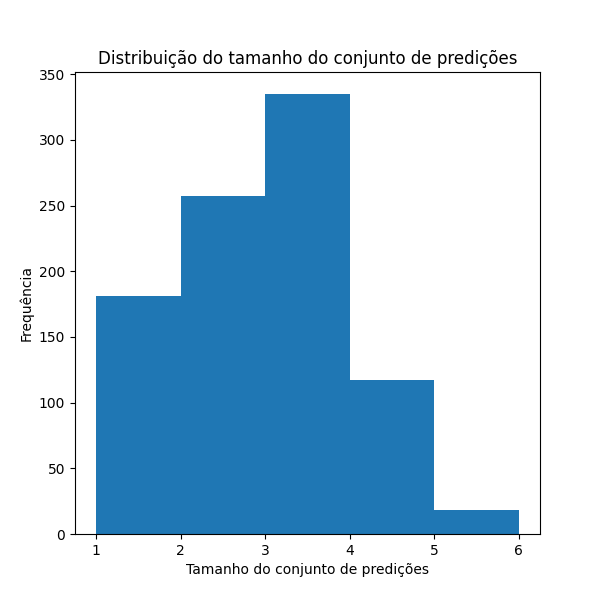
\includegraphics[width=0.25\textwidth]{figs/conformal_prediction/densenet169_cp_corn.png} \\ \hline
    \end{tabular}
    \caption{Histograma do tamanho dos conjuntos de predição para cinco modelos relevantes.}
    \label{tab:cp_set_sizes}
\end{table}

Em contraste, a abordagem ordinal com uso do CORN produziu conjuntos de predição muito mais informativos e úteis. A principal vantagem foi o número de conjuntos de tamanho um, indicando alta confiança do modelo em muitos casos. Por exemplo, os modelos Inception-v3 e DenseNet-169 geraram 198 e 181 predições únicas, respectivamente. Isso representa aproximadamente 20\% do conjunto de teste recebendo uma resposta precisa. Os histogramas mostram uma distribuição mais deslocada para a esquerda, ou seja, conjuntos menores.

Portanto, para uma ferramenta de suporte à decisão clínica, a abordagem baseada em CORN é superior. Um radiologista se beneficiaria muito mais de um sistema que frequentemente fornece uma resposta única e acionável, mesmo que a garantia de cobertura seja ligeiramente menos rígida, do que de um sistema que quase sempre responde com um conjunto de três a quatro possibilidades. A abordagem ordinal traduz melhor a confiança do modelo em resultados práticos e clinicamente relevantes.

\section{Interpretabilidade dos Modelos}

Para garantir que o desempenho quantitativo dos modelos seja acompanhado de um processo de decisão clinicamente relevante, foi realizada uma análise qualitativa utilizando a técnica de Grad-CAM. A análise revelou padrões consistentes e distintos entre as arquiteturas, reforçando a confiabilidade dos modelos de melhor desempenho. A \autoref{tab:gradcams_top5_models} ilustra as Grad-CAMs para os modelos que tiveram o melhor desempenho preditivo.

Uma observação fundamental foi que os modelos de modo geral focaram sua atenção em regiões cruciais para o diagnóstico da OA, como o espaço articular. Por exemplo, como ilustrado na \autoref{tab:gradcams_top5_models}, para uma classificação correta de KL-3 (moderado), o mapa de calor evidencia uma forte ativação sobre o espaço articular com o menor estreitamento (lado esquerdo da radiografia). Esse comportamento foi observado na grande maioria das predições corretas, indicando que os modelos não apenas acertaram a classe, mas o fizeram com base nos mesmos indicadores visuais que um radiologista utilizaria, aumentando a confiança em sua validade clínica.

Além disso, o Grad-CAM revelou estratégias visuais distintas entre as RNCs e os ViTs. Para a mesma radiografia de entrada, as RNCs tenderam a produzir mapas de calor mais focados e localizados. Sua atenção se concentrou onde existem bordas de alta frequência, ou seja, nos espaços articulares. Isso reflete o forte viés indutivo das convoluções para a detecção desses padrões locais.

Por outro lado, os ViTs geraram mapas de calor mais difusos e contextuais. Em vez de focar em um único ponto, a atenção frequentemente se espalhou por uma região mais ampla, como é o caso dos modelos DaViT-B e GCViT-B. Isso também está alinhado com a capacidade dos transformers de modelar relações de longo alcance numa imagem.

Em síntese, a análise de interpretabilidade com Grad-CAM não só validou que os modelos de alto desempenho aprenderam a identificar características patológicas clinicamente relevantes da OA de joelho, mas também ofereceu uma análise sobre as diferentes estratégias de análise visual das arquiteturas. Tanto RNCs quanto ViTs se mostraram eficazes para a classificação correta com base em características visuais adequadas e podem ser utilizadas como ferramenta de suporte na análise clínica para diagnosticar a severidade da OA de joelho.

\begin{sidewaystable}[!htbp]
    \centering
    \begin{tabular}{|c|c|c|c|c|c|}
        \hline
        \textbf{Modelo} & \textbf{KL-0} & \textbf{KL-1} & \textbf{KL-2} & \textbf{KL-3} & \textbf{KL-4} \\ \hline
        DenseNet-169 & 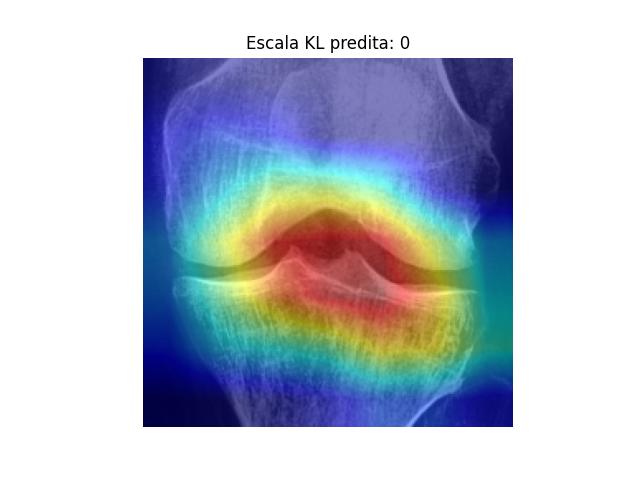
\includegraphics[width=0.15\textwidth]{figs/gradcams/gradcam_densenet169_kl0.png} & 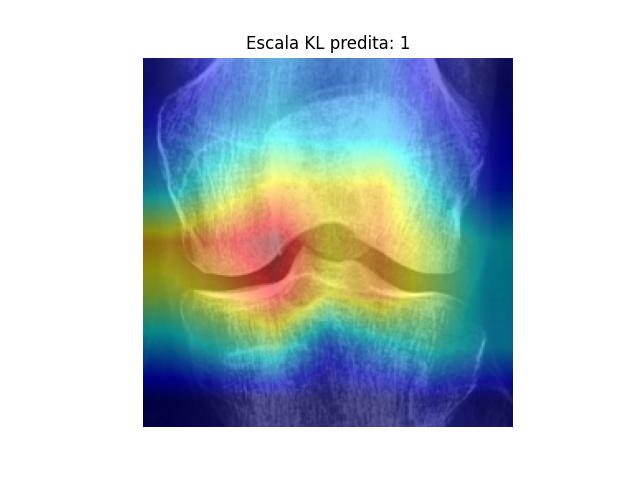
\includegraphics[width=0.15\textwidth]{figs/gradcams/gradcam_densenet169_kl1.png} & 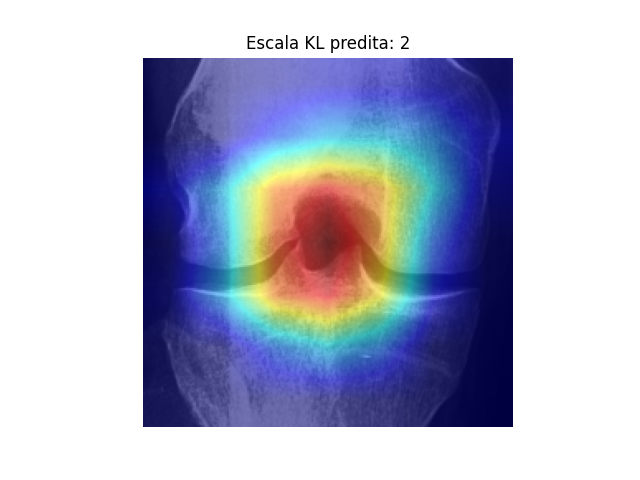
\includegraphics[width=0.15\textwidth]{figs/gradcams/gradcam_densenet169_kl2.png} & 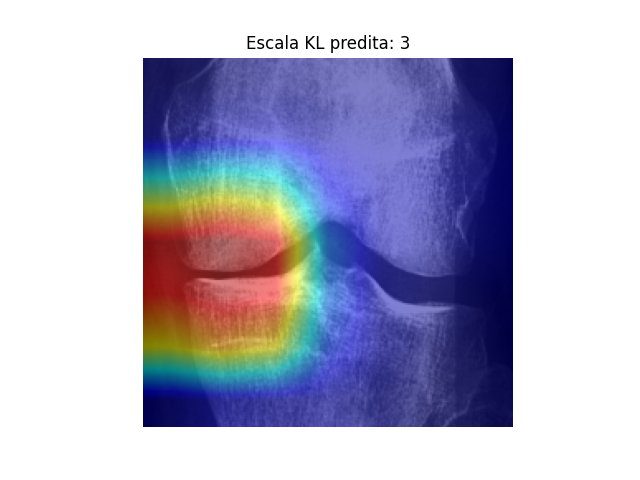
\includegraphics[width=0.15\textwidth]{figs/gradcams/gradcam_densenet169_kl3.png} & 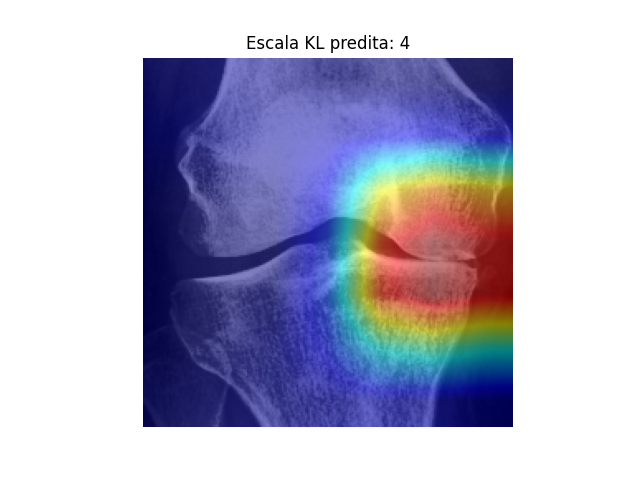
\includegraphics[width=0.15\textwidth]{figs/gradcams/gradcam_densenet169_kl4.png} \\ \hline
        DenseNet-121 & 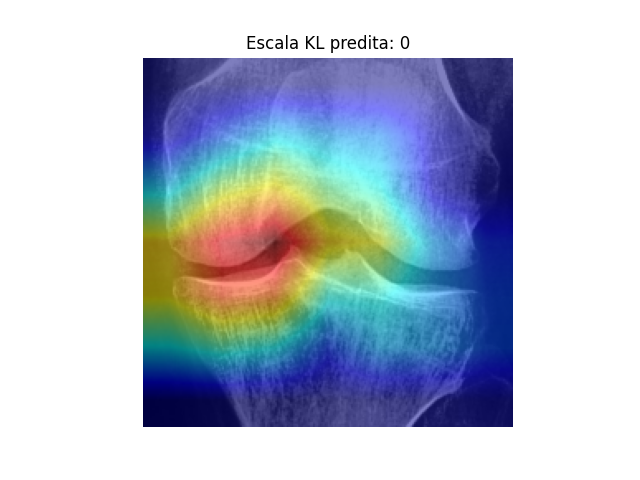
\includegraphics[width=0.15\textwidth]{figs/gradcams/gradcam_densenet121_kl0.png} & 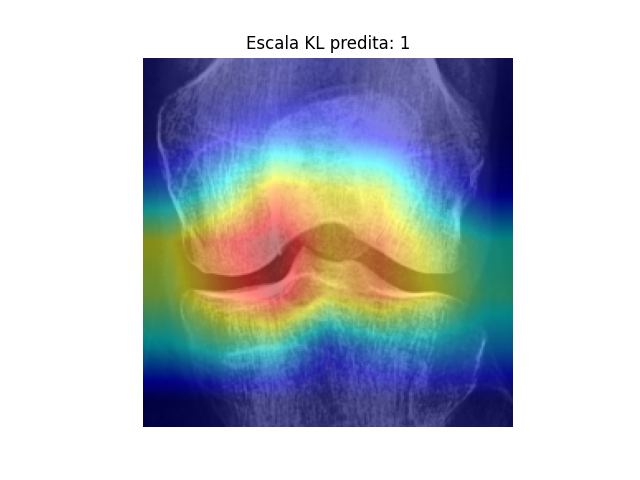
\includegraphics[width=0.15\textwidth]{figs/gradcams/gradcam_densenet121_kl1.png} & 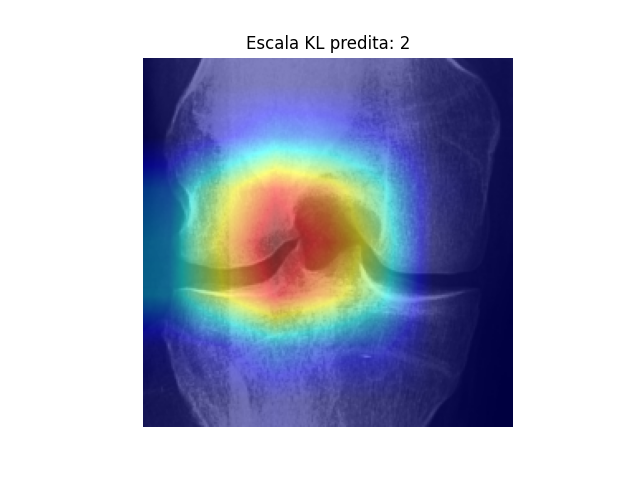
\includegraphics[width=0.15\textwidth]{figs/gradcams/gradcam_densenet121_kl2.png} & 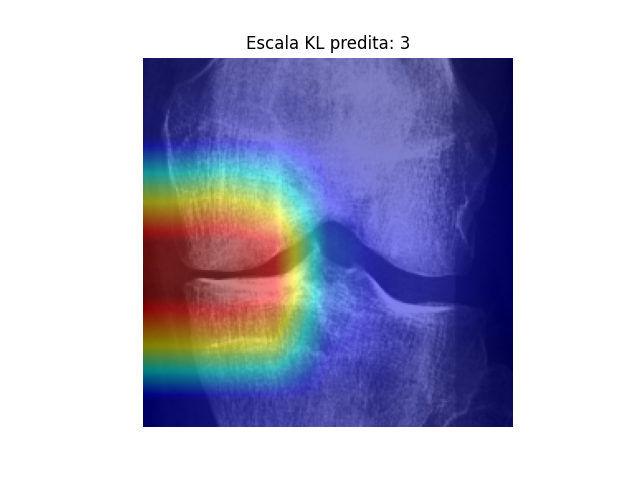
\includegraphics[width=0.15\textwidth]{figs/gradcams/gradcam_densenet121_kl3.png} & 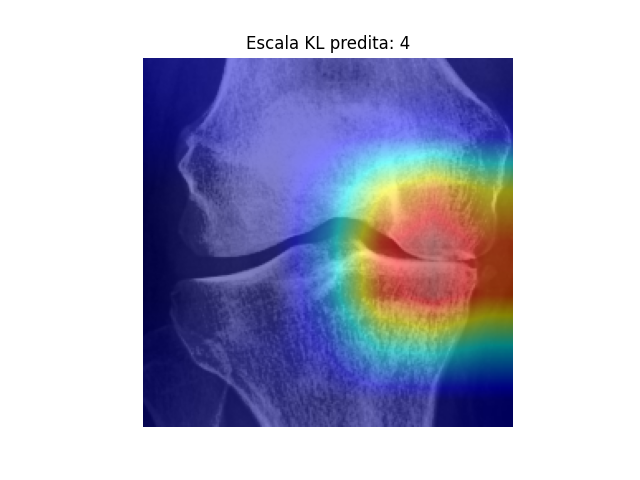
\includegraphics[width=0.15\textwidth]{figs/gradcams/gradcam_densenet121_kl4.png} \\ \hline
        DaViT-B & 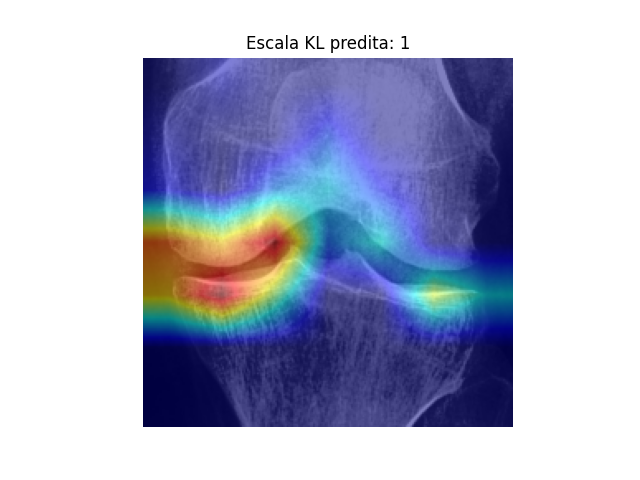
\includegraphics[width=0.15\textwidth]{figs/gradcams/gradcam_davit_kl0.png} & 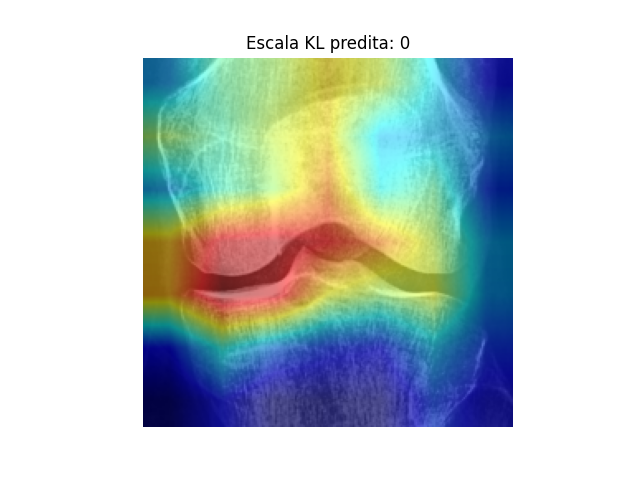
\includegraphics[width=0.15\textwidth]{figs/gradcams/gradcam_davit_kl1.png} & 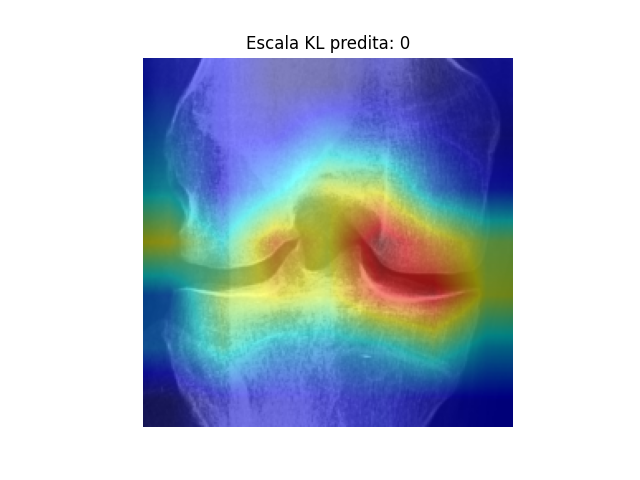
\includegraphics[width=0.15\textwidth]{figs/gradcams/gradcam_davit_kl2.png} & 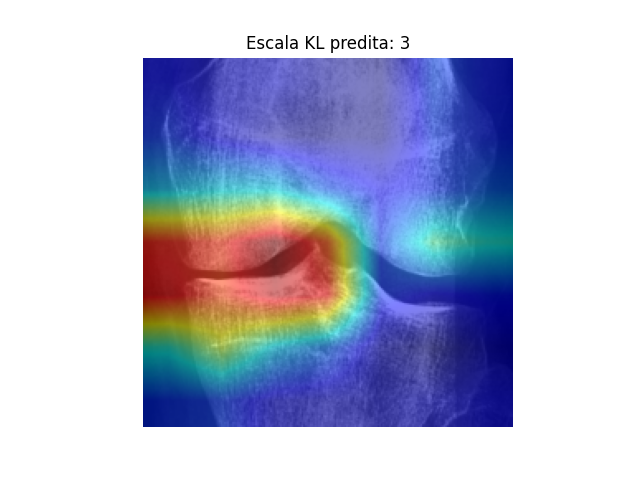
\includegraphics[width=0.15\textwidth]{figs/gradcams/gradcam_davit_kl3.png} & 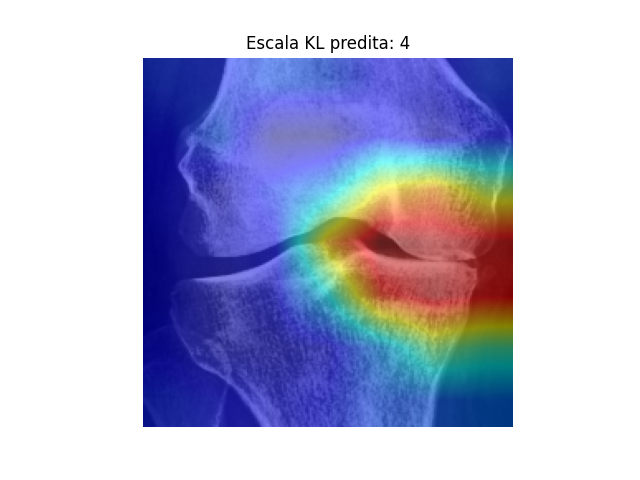
\includegraphics[width=0.15\textwidth]{figs/gradcams/gradcam_davit_kl4.png} \\ \hline
        GCViT-B & 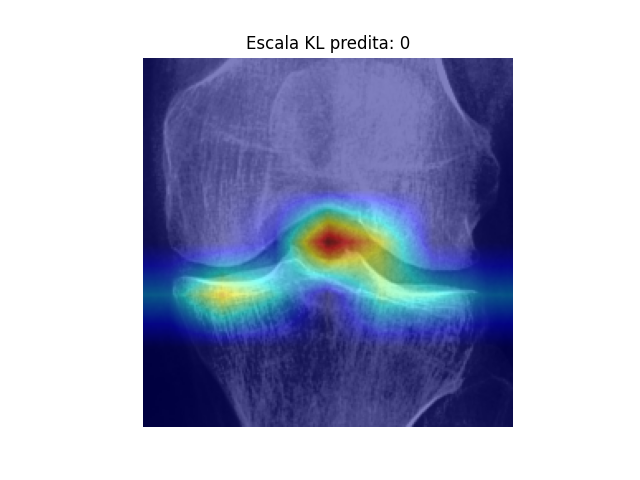
\includegraphics[width=0.15\textwidth]{figs/gradcams/gradcam_gcvit_kl0.png} & 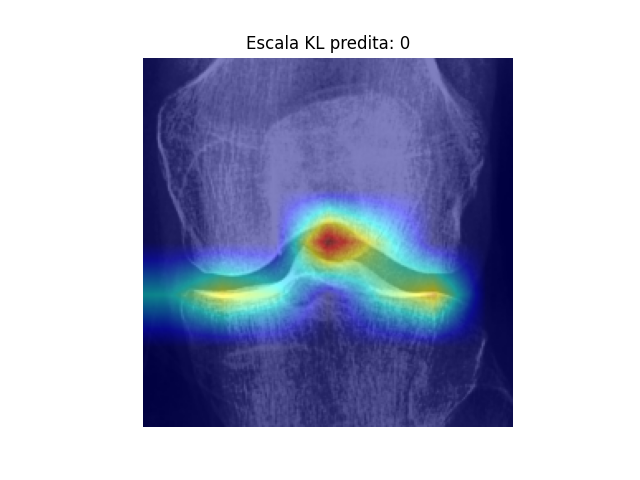
\includegraphics[width=0.15\textwidth]{figs/gradcams/gradcam_gcvit_kl1.png} & 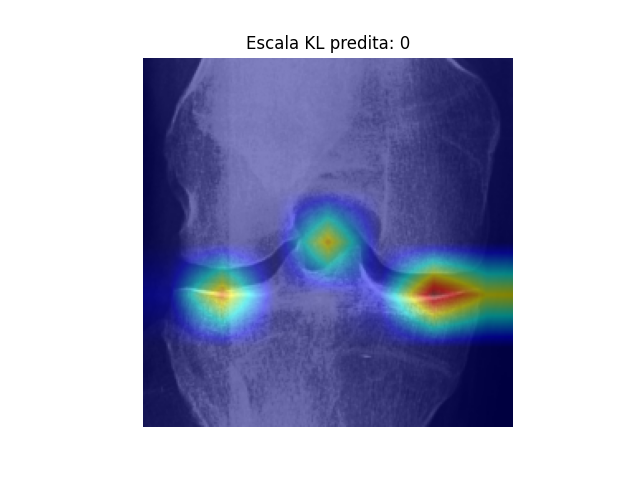
\includegraphics[width=0.15\textwidth]{figs/gradcams/gradcam_gcvit_kl2.png} & 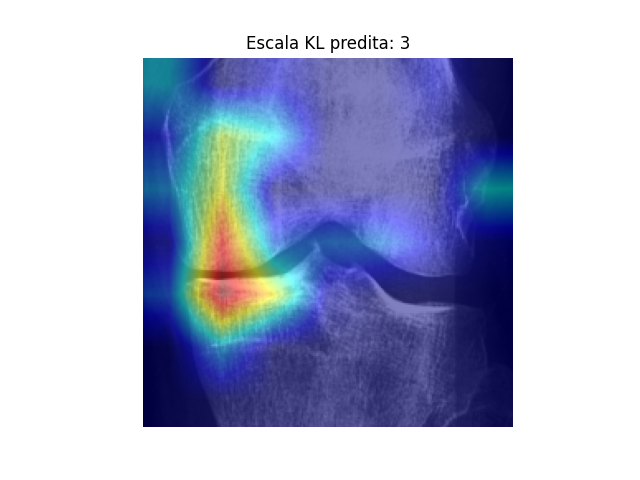
\includegraphics[width=0.15\textwidth]{figs/gradcams/gradcam_gcvit_kl3.png} & 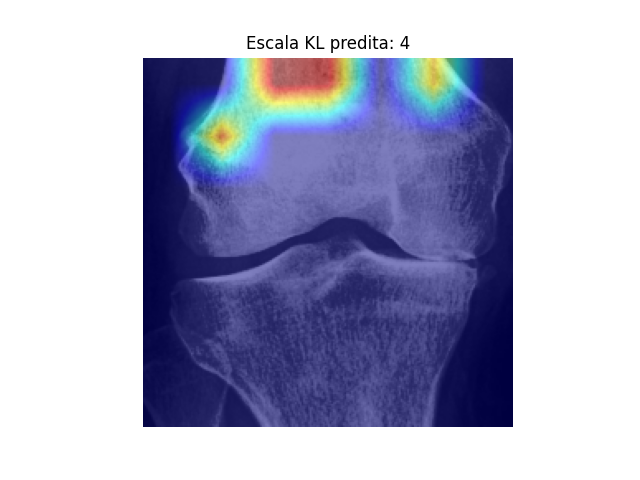
\includegraphics[width=0.15\textwidth]{figs/gradcams/gradcam_gcvit_kl4.png} \\ \hline
        Inception-v3 & \includegraphics[width=0.15\textwidth]{figs/gradcams/gradcam_inceptionv3_kl0.png} & \includegraphics[width=0.15\textwidth]{figs/gradcams/gradcam_inceptionv3_kl1.png} & \includegraphics[width=0.15\textwidth]{figs/gradcams/gradcam_inceptionv3_kl2.png} & \includegraphics[width=0.15\textwidth]{figs/gradcams/gradcam_inceptionv3_kl3.png} & \includegraphics[width=0.15\textwidth]{figs/gradcams/gradcam_inceptionv3_kl4.png} \\ \hline
    \end{tabular}
    \caption{Visualização Grad-CAM para os cinco principais modelos.}
    \label{tab:gradcams_top5_models}
\end{sidewaystable}